\documentclass[preprint,12pt,authoryear]{elsarticle}
\usepackage[letterpaper,margin=1in]{geometry}
\usepackage[UTF8,fontset=fandol,heading=false,scheme=chinese]{ctex}
\usepackage{amsmath,amssymb,amsfonts,bm}
\usepackage{graphicx}
\usepackage{longtable,booktabs,array,calc}
\usepackage{xcolor}
\usepackage{pdflscape}
\usepackage[hidelinks]{hyperref}
\usepackage{newunicodechar}
\newunicodechar{→}{\ensuremath{\rightarrow}}
\newunicodechar{⁻}{\textsuperscript{-}}
\newunicodechar{⁵}{\textsuperscript{5}}
\newunicodechar{·}{\textperiodcentered}
\newunicodechar{×}{\ensuremath{\times}}
\newunicodechar{−}{\ensuremath{-}}
\newunicodechar{⊗}{\ensuremath{\otimes}}
\newunicodechar{≤}{\ensuremath{\leq}}
\providecommand{\tightlist}{\setlength{\itemsep}{0pt}\setlength{\parskip}{0pt}}
\makeatletter
\newsavebox\pandoc@box
\newcommand*\pandocbounded[1]{\sbox\pandoc@box{#1}%
  \Gscale@div\@tempa{\textheight}{\dimexpr\ht\pandoc@box+\dp\pandoc@box\relax}%
  \Gscale@div\@tempb{\linewidth}{\wd\pandoc@box}%
  \ifdim\@tempb\p@<\@tempa\p@\let\@tempa\@tempb\fi
  \ifdim\@tempa\p@<\p@\scalebox{\@tempa}{\usebox\pandoc@box}\else\usebox{\pandoc@box}\fi}
\makeatother
\def\LTcaptype{table}
\setlength{\LTleft}{0pt}\setlength{\LTright}{0pt}\setlength{\LTcapwidth}{\linewidth}
\setlength{\emergencystretch}{3em}
\journal{Computer Methods in Applied Mechanics and Engineering}
\newunicodechar{⪯}{\ensuremath{\preceq}}\newunicodechar{⪰}{\ensuremath{\succeq}}
\newunicodechar{δ}{\ensuremath{\delta}}\newunicodechar{κ}{\ensuremath{\kappa}}
\abstracttitle{摘要}\keywordtitle{关键词}
\linespread{1.25}
\setcounter{secnumdepth}{0}
\renewcommand{\thefigure}{S\ifnum\value{figure}<10 0\fi\arabic{figure}}
\begin{document}
\begin{center}{\Large 补充材料}\\[4pt]{\Large\bfseries NICE：带平衡校正的神经初始化静力凝聚及其在切割 TPMS 点阵厚度设计中的应用}\end{center}

补充说明、补充表和补充图按其在本补充材料中出现的顺序编号。变体标签与正文（表 2）一致。未修正延续与平滑训练两个变体未列入该表，其结果在本补充材料中给出。下方索引给出各变体在数据存档中的记录标识符。

\section{R1. 变体与几何索引}

{\def\LTcaptype{none} % do not increment counter
{\small
\begin{longtable}[]{@{}
  >{\raggedright\arraybackslash}p{(\linewidth - 4\tabcolsep) * \real{0.3333}}
  >{\raggedright\arraybackslash}p{(\linewidth - 4\tabcolsep) * \real{0.3333}}
  >{\raggedright\arraybackslash}p{(\linewidth - 4\tabcolsep) * \real{0.3333}}@{}}
\toprule\noalign{}
\begin{minipage}[b]{\linewidth}\raggedright
标签
\end{minipage} & \begin{minipage}[b]{\linewidth}\raggedright
数值作用
\end{minipage} & \begin{minipage}[b]{\linewidth}\raggedright
数据存档中的记录标识符
\end{minipage} \\
\midrule\noalign{}
\endhead
\bottomrule\noalign{}
\endlastfoot
基础网络 & 基线变体；所有继续训练以及第 5.5 节修正实验的初始网络参数 & v2L1 \\
未修正延续 & 由基础网络继续训练；训练和评估中均不施加修正 & A0\_ctrl \\
平滑训练 & 由基础网络继续训练，训练时施加八步光滑 & A2b\_tail8 \\
基础网络加修正 & 部署时对基础网络施加 NICE 的修正，不重新训练 & B2grid \\
NICE & 主要变体，训练时施加完整修正（8 / Q1(17) / 8） & A3\_2grid \\
\end{longtable}}
}

{\def\LTcaptype{none} % do not increment counter
{\small
\begin{longtable}[]{@{}
  >{\raggedright\arraybackslash}p{(\linewidth - 4\tabcolsep) * \real{0.3333}}
  >{\raggedright\arraybackslash}p{(\linewidth - 4\tabcolsep) * \real{0.3333}}
  >{\raggedright\arraybackslash}p{(\linewidth - 4\tabcolsep) * \real{0.3333}}@{}}
\toprule\noalign{}
\begin{minipage}[b]{\linewidth}\raggedright
胞元标签
\end{minipage} & \begin{minipage}[b]{\linewidth}\raggedright
切割程度分组
\end{minipage} & \begin{minipage}[b]{\linewidth}\raggedright
数据存档中的几何标识符
\end{minipage} \\
\midrule\noalign{}
\endhead
\bottomrule\noalign{}
\endlastfoot
U1 & 未切割 & fresh\_val\_2000\_full \\
U2 & 未切割 & fresh\_val\_2001\_full \\
M1 & 中度切割 & fresh\_val\_2003\_d1\_v1 \\
H1 & 重度切割 & fresh\_val\_2005\_d1\_v0 \\
M2 & 中度切割 & fresh\_val\_2006\_d0\_v1 \\
H2 & 重度切割 & fresh\_val\_2010\_d0\_v0 \\
H3 & 重度切割 & fresh\_val\_2002\_d0\_v0 \\
L1 & 轻度切割 & fresh\_val\_2004\_d0\_v2 \\
W1：NICE 误差最大的验证胞元（表 ST08b、ST10） & 中度切割 & fresh\_val\_2051\_d1\_v1 \\
W2（表 ST08b） & 重度切割 & fresh\_val\_2045\_d1\_v0 \\
W3：壁最薄的验证胞元（表 ST08b、ST10） & 重度切割 & fresh\_val\_2074\_d0\_v0 \\
W4（表 ST08b） & 重度切割 & fresh\_val\_2021\_d1\_v0 \\
W5（表 ST08b） & 轻度切割 & fresh\_val\_2063\_d1\_v2 \\
RU（表 ST08b） & 未切割 & fresh\_val\_2032\_full \\
RL（表 ST08b） & 轻度切割 & fresh\_val\_2047\_d1\_v2 \\
RM（表 ST08b） & 中度切割 & fresh\_val\_2078\_d0\_v1 \\
RH（表 ST08b） & 重度切割 & fresh\_val\_2053\_d1\_v0 \\
\end{longtable}}
}

在验证胞元标识符中，d0 和 d1 表示切割角 \(\vartheta\) 位于 \((0,\pi/4)\) 的哪一半区间，v0、v1 和 v2 分别表示按剩余体积划分的重度、中度和轻度切割程度分组。在 U1/x 等构型标签中，x 和 y 表示图 9 中的相邻胞元构型。部署几何采用表 ST13 的 G1--G4 标签，下表给出它们在数据存档中的标识符。

{\def\LTcaptype{none} % do not increment counter
{\small
\begin{longtable}[]{@{}lll@{}}
\toprule\noalign{}
基准标签 & 切割程度分组 & 数据存档中的几何标识符 \\
\midrule\noalign{}
\endhead
\bottomrule\noalign{}
\endlastfoot
G1 & 切割 & fresh\_train\_0020\_cover01\_r2 \\
G2 & 切割 & fresh\_train\_0020\_cover01\_r1 \\
G3 & 未切割 & fresh\_train\_0020\_full \\
G4 & 未切割 & fresh\_train\_0007\_full \\
\end{longtable}}
}

\section{表 ST01. 训练与评估设置}

{\def\LTcaptype{none} % do not increment counter
{\footnotesize
\begin{longtable}[]{@{}
  >{\raggedright\arraybackslash}p{(\linewidth - 12\tabcolsep) * \real{0.1429}}
  >{\raggedright\arraybackslash}p{(\linewidth - 12\tabcolsep) * \real{0.1429}}
  >{\raggedright\arraybackslash}p{(\linewidth - 12\tabcolsep) * \real{0.1429}}
  >{\raggedright\arraybackslash}p{(\linewidth - 12\tabcolsep) * \real{0.1429}}
  >{\raggedright\arraybackslash}p{(\linewidth - 12\tabcolsep) * \real{0.1429}}
  >{\raggedright\arraybackslash}p{(\linewidth - 12\tabcolsep) * \real{0.1429}}
  >{\raggedright\arraybackslash}p{(\linewidth - 12\tabcolsep) * \real{0.1429}}@{}}
\toprule\noalign{}
\begin{minipage}[b]{\linewidth}\raggedright
变体
\end{minipage} & \begin{minipage}[b]{\linewidth}\raggedright
训练集（几何数）
\end{minipage} & \begin{minipage}[b]{\linewidth}\raggedright
训练期验证几何
\end{minipage} & \begin{minipage}[b]{\linewidth}\raggedright
训练步数
\end{minipage} & \begin{minipage}[b]{\linewidth}\raggedright
评估的训练步 / 参数
\end{minipage} & \begin{minipage}[b]{\linewidth}\raggedright
评估时修正
\end{minipage} & \begin{minipage}[b]{\linewidth}\raggedright
评估取向
\end{minipage} \\
\midrule\noalign{}
\endhead
\bottomrule\noalign{}
\endlastfoot
基础网络 & 305 & 40 & 40,000 & 30,000 / EMA & 无 & 恒等、17 \\
未修正延续 & 591 & 40 & 15,000 & 15,000 / EMA & 无 & 恒等 \\
平滑训练 & 591 & 40 & 15,000 & 15,000 / EMA & 八步光滑 & 恒等 \\
基础网络加修正 & 305 & 40 & --- & 30,000 / EMA & 8 / Q1(17) / 8 & 恒等 \\
NICE & 591 & 40 & 15,000 & 15,000 / EMA & 8 / Q1(17) / 8 & 恒等、17 \\
\end{longtable}}
}

所有变体均在表 ST02 的 80 个验证几何上评估。取向 17 是附录 G（式 (G.2)）中 48 个立方体对称变换之一，同时作用于几何和测试位移；取向 0 为恒等变换。591 个几何的训练集包括基础网络 305 个训练几何中的 304 个（移除了一个近似为机构的胞元），以及另外 287 个训练几何。按下文所述的几何替换方式，每次 15,000 步的继续训练至多访问其 591 个训练几何中的 153 个；基础网络在 40,000 个训练步中访问了自身全部 305 个几何。未修正延续、平滑训练和 NICE 使用相同的随机种子和数据划分，因此按相同顺序抽取几何。

训练设置（表 2 中各变体以及未修正延续和平滑训练通用）：

\begin{itemize}
\tightlist
\item
  每批 16 个测试位移，每一步更换几何。训练集中的三个几何驻留在 GPU 上，每 100 步替换其中一个，因此一次 \(N_{\rm st}\) 步的训练至多访问 \(N_{\rm st}/100+3\) 个不同的训练几何。
\item
  名义类别权重按 \texttt{force}、\texttt{force\_c}、\texttt{support}、\texttt{support\_k}、\texttt{face}、\texttt{face\_c}、\texttt{macro}、\texttt{grf}、\texttt{glued}、\texttt{adv} 的顺序依次为 \(0.10,0.10,0.075,0.075,0.10,0.10,0.10,0.125,0.075,0.15\)。这些权重在可用类别上重新归一化，并按系统配额分配。
\item
  采用 Adam 优化器与单周期学习率调度：峰值 \(3\times10^{-4}\)，5\% 预热，余弦衰减，最终除数因子为 100；梯度范数裁剪阈值为 1。
\item
  模型选择和评估使用网络参数的指数移动平均（EMA），衰减率为 0.9997，并进行零初始化偏差校正。
\item
  式 (13)：能量项对数的自变量以 \(10^{-12}\) 为下限截断；灵敏度项权重为 1。
\end{itemize}

计至最后一个训练步，基础网络的训练在 GPU 上（第 5.1 节）耗时 4.6 h，NICE 的继续训练耗时 3.5 h；若计入全部选择评估，则分别为 5.0 h 和 4.8 h。训练期间 GPU 峰值显存为 29.6 GiB。基础网络由此前三个训练阶段（合计 7.5 GPU 小时）得到的参数初始化。NICE 的离线成本约为 60 GPU 小时，包括这些阶段、上述两次运行（含其选择评估），以及测试位移集与精确灵敏度的生成。后者涵盖数据划分中的 691 个几何，即 591 个训练几何和 100 个验证几何（验证几何包括表 ST02 的 80 个），耗时约 42 GPU 小时（第 5.1 节）。

对于基础网络、未修正延续、平滑训练和 NICE，检查点选择使用经偏差校正的 EMA 参数，并同时采用恒等取向（\(v=0\)）和取向 17（\(v=17\)），而表 ST03 仅报告恒等取向。几何族由训练期验证列表中同一厚度场生成的几何组成；独立生成的验证胞元自成一族。在几何族 \(f\) 和取向 \(v\) 内，记 \(\bar\varepsilon_{fv}\) 为平均能量误差在各选择类别上的平均值，\(\bar e_{s,fv}\) 为带灵敏度标签类别的平均相对灵敏度向量误差，\(\varepsilon^{(90)}_{fv}\) 为各测试位移能量误差第 90 百分位数的类别平均。每个类别统计量先在该族的可用几何上取平均。选择得分为

\[
J_{\rm sel}=\frac12\sum_{v\in\{0,17\}}\frac1{|\mathcal F|}
\sum_{f\in\mathcal F}\left(\bar\varepsilon_{fv}+\bar e_{s,fv}+\tfrac12\varepsilon^{(90)}_{fv}\right).
\]

各族与两个取向的权重相同。八个选择类别为 \texttt{force}、\texttt{support}、\texttt{face}、\texttt{macro}、\texttt{grf}、\texttt{force\_c}、\texttt{face\_c} 和 \texttt{support\_k}；缺失的类别略去，缺失的灵敏度项记为零。在符合条件的评估中，选取有限得分最低者。

\begin{itemize}
\tightlist
\item
  基础网络在第 10,000、20,000、30,000 和 40,000 个训练步评分（\(J_{\rm sel}\) = 0.1057、0.1065、0.0905 和 0.0912），选定第 30,000 步的参数。所有继续训练的变体均从这些参数出发。
\item
  未修正延续和 NICE 在第 7,500 和 15,000 个训练步评分（0.0944 和 0.0906；0.00281 和 0.00237）；两者均为最终参数得分较低，因而选用最终参数。
\item
  平滑训练采用相同的评估计划和取向；该变体的选择得分未记录，采用最终步（第 15,000 步）的参数。
\item
  在所有变体于 80 个验证几何和两胞元构型上完成比较之后，NICE 被确定为主要变体。
\end{itemize}

80 个验证几何中有 20 个（6 个未切割、14 个切割）属于选择列表，其中包括补充材料第 R1 节中全部八个用于详细比较的胞元。

\section{表 ST02. 验证几何域}

这 80 个几何采用独立生成的厚度场，其中 20 个为均匀场、30 个为仿射场、30 个为混合三线性场。生成器将每个角点参数约束在 \([0.17520160,0.69933962]\) 内，角点参数跨度至多为 0.47，参考坐标下梯度范数的最大值至多为 0.47。每八个几何为一组，组内对均匀场等效的中心体积分数在 0.1 与 0.4 之间分层抽样；非均匀的仿射或三线性形状在上述约束内缩放。该中心密度参数仅为采样坐标，并非切割后的材料分数。

标准切割法向为 \((\cos\vartheta,\sin\vartheta,0)\)。生成器在 \((0,\pi/4)\) 的两个半区间上对 \(\vartheta\) 分层抽样，并在 \((0,1)\) 的三个三等分区间上对切割后剩余的胞元立方体体积 \(v_{\mathcal B}\) 分层抽样。每八个验证场中有两个未切割，其余六个覆盖各角度--体积组合。训练集与验证集取自相互独立的随机流；本表描述的是 80 个几何的验证集。

{\def\LTcaptype{none} % do not increment counter
{\small
\begin{longtable}[]{@{}
  >{\raggedright\arraybackslash}p{(\linewidth - 8\tabcolsep) * \real{0.1875}}
  >{\raggedleft\arraybackslash}p{(\linewidth - 8\tabcolsep) * \real{0.2500}}
  >{\raggedright\arraybackslash}p{(\linewidth - 8\tabcolsep) * \real{0.1875}}
  >{\raggedright\arraybackslash}p{(\linewidth - 8\tabcolsep) * \real{0.1875}}
  >{\raggedright\arraybackslash}p{(\linewidth - 8\tabcolsep) * \real{0.1875}}@{}}
\toprule\noalign{}
\begin{minipage}[b]{\linewidth}\raggedright
切割程度分组
\end{minipage} & \begin{minipage}[b]{\linewidth}\raggedleft
几何数
\end{minipage} & \begin{minipage}[b]{\linewidth}\raggedright
\(v_{\mathcal B}\) 的生成区间
\end{minipage} & \begin{minipage}[b]{\linewidth}\raggedright
观测 \(v_{\mathcal B}\)
\end{minipage} & \begin{minipage}[b]{\linewidth}\raggedright
观测角点参数范围
\end{minipage} \\
\midrule\noalign{}
\endhead
\bottomrule\noalign{}
\endlastfoot
未切割 & 20 & 1 & 1 & 0.1762--0.6902 \\
轻度切割 & 20 & \((2/3,1)\) & 0.6765--0.9996 & 0.1853--0.6972 \\
中度切割 & 20 & \((1/3,2/3)\) & 0.3437--0.6605 & 0.1867--0.6983 \\
重度切割 & 20 & \((0,1/3)\) & 0.01326--0.3195 & 0.1768--0.6946 \\
\end{longtable}}
}

切割体积指胞元立方体与 TPMS 带求交之前的体积。任意两个验证几何在立方体对称变换下均不重合。在 \(n=32\) 时，80 个几何的主自由度数中位数为 23,604，范围为 2,679 至 45,900；激活自由度数中位数为 221,442，范围为 2,757 至 439,092。用于谱分析和装配的算例在补充材料第 R1 节的几何索引中标明；它们作为测试算例报告，不构成用于总体推断的随机样本。

\section{表 ST03. 各载荷类别的能量误差（恒等取向）}

表中条目为几何间的均值 / 最大值，单位为百分比：每个几何先对其测试位移取平均，各几何等权。该最大值并非最差的单个测试位移。``基础网络加修正''指部署时对基础网络施加 NICE 的修正、不重新训练所得的变体。最后一列将 NICE 限于既未参与训练、也未参与检查点选择的 60 个验证几何（另外 20 个参与了检查点选择，表 ST01）。在面力载荷下，NICE 在 80 个几何的 5,120 个单独采样测试位移上的第 95 百分位数为 0.331\%，第 99 百分位数为 0.693\%，最大值为 1.24\%。检查点选择之外 60 个几何的 3,840 个测试位移上，相应数值为 0.355\%、0.734\% 和 1.24\%。在面力载荷下，基础网络加修正的均值为 0.0965\%，NICE 为 0.0737\%，比值为 1.31。对 80 个几何进行有放回重抽样（配对、几何等权均值之比、百分位区间），所得 95\% 区间为 1.20--1.40。

{\def\LTcaptype{none} % do not increment counter
{\scriptsize
\begin{longtable}[]{@{}
  >{\raggedright\arraybackslash}p{(\linewidth - 14\tabcolsep) * \real{0.1250}}
  >{\raggedright\arraybackslash}p{(\linewidth - 14\tabcolsep) * \real{0.1250}}
  >{\raggedright\arraybackslash}p{(\linewidth - 14\tabcolsep) * \real{0.1250}}
  >{\raggedright\arraybackslash}p{(\linewidth - 14\tabcolsep) * \real{0.1250}}
  >{\raggedright\arraybackslash}p{(\linewidth - 14\tabcolsep) * \real{0.1250}}
  >{\raggedright\arraybackslash}p{(\linewidth - 14\tabcolsep) * \real{0.1250}}
  >{\raggedright\arraybackslash}p{(\linewidth - 14\tabcolsep) * \real{0.1250}}
  >{\raggedright\arraybackslash}p{(\linewidth - 14\tabcolsep) * \real{0.1250}}@{}}
\toprule\noalign{}
\begin{minipage}[b]{\linewidth}\raggedright
类别
\end{minipage} & \begin{minipage}[b]{\linewidth}\raggedright
几何数（全部 / 选择之外）
\end{minipage} & \begin{minipage}[b]{\linewidth}\raggedright
基础网络
\end{minipage} & \begin{minipage}[b]{\linewidth}\raggedright
未修正延续
\end{minipage} & \begin{minipage}[b]{\linewidth}\raggedright
平滑训练
\end{minipage} & \begin{minipage}[b]{\linewidth}\raggedright
基础网络加修正
\end{minipage} & \begin{minipage}[b]{\linewidth}\raggedright
NICE
\end{minipage} & \begin{minipage}[b]{\linewidth}\raggedright
NICE（选择之外）
\end{minipage} \\
\midrule\noalign{}
\endhead
\bottomrule\noalign{}
\endlastfoot
force & 80 / 60 & 5.036 / 70.122 & 4.607 / 62.465 & 0.525 / 3.658 & 0.092 / 0.683 & 0.058 / 0.325 & 0.059 / 0.325 \\
support & 80 / 60 & 5.332 / 99.857 & 4.878 / 90.741 & 0.638 / 3.552 & 0.084 / 0.852 & 0.055 / 0.372 & 0.056 / 0.372 \\
face & 80 / 60 & 2.486 / 22.139 & 2.233 / 17.635 & 0.165 / 1.808 & 0.072 / 1.990 & 0.037 / 0.724 & 0.040 / 0.724 \\
macro & 80 / 60 & 0.842 / 2.636 & 0.827 / 2.584 & 0.203 / 0.935 & 0.022 / 0.165 & 0.015 / 0.118 & 0.015 / 0.118 \\
grf & 80 / 60 & 2.038 / 4.582 & 2.009 / 4.550 & 0.251 / 0.933 & 0.029 / 0.180 & 0.025 / 0.143 & 0.025 / 0.143 \\
force\_c & 80 / 60 & 6.886 / 48.628 & 6.334 / 41.962 & 1.280 / 7.817 & 0.097 / 0.905 & 0.074 / 0.651 & 0.077 / 0.651 \\
face\_c & 80 / 60 & 3.150 / 36.337 & 2.806 / 25.525 & 0.483 / 2.326 & 0.043 / 0.319 & 0.032 / 0.210 & 0.033 / 0.210 \\
support\_k & 75 / 56 & 4.177 / 28.817 & 3.941 / 26.175 & 0.938 / 5.246 & 0.077 / 0.632 & 0.057 / 0.468 & 0.058 / 0.468 \\
glued & 75 / 60 & 4.593 / 38.128 & 4.422 / 42.030 & 0.953 / 4.629 & 0.078 / 0.555 & 0.060 / 0.384 & 0.055 / 0.384 \\
\end{longtable}}
}

在面力载荷下，NICE 在检查点选择之外 60 个几何上各切割程度分组的均值为 0.020\%（未切割）、0.054\%（轻度）、0.105\%（中度）和 0.126\%（重度）。80 个几何中单个几何平均误差最大的五个值（0.651\%、0.540\%、0.487\%、0.303\%、0.287\%）均属于这 60 个几何。

\subsection{ST03b. 集中节点载荷与面力载荷下各切割程度分组的均值（\%）}

{\def\LTcaptype{none} % do not increment counter
{\footnotesize
\begin{longtable}[]{@{}
  >{\raggedright\arraybackslash}p{(\linewidth - 12\tabcolsep) * \real{0.1429}}
  >{\raggedright\arraybackslash}p{(\linewidth - 12\tabcolsep) * \real{0.1429}}
  >{\raggedright\arraybackslash}p{(\linewidth - 12\tabcolsep) * \real{0.1429}}
  >{\raggedright\arraybackslash}p{(\linewidth - 12\tabcolsep) * \real{0.1429}}
  >{\raggedright\arraybackslash}p{(\linewidth - 12\tabcolsep) * \real{0.1429}}
  >{\raggedright\arraybackslash}p{(\linewidth - 12\tabcolsep) * \real{0.1429}}
  >{\raggedright\arraybackslash}p{(\linewidth - 12\tabcolsep) * \real{0.1429}}@{}}
\toprule\noalign{}
\begin{minipage}[b]{\linewidth}\raggedright
切割程度分组
\end{minipage} & \begin{minipage}[b]{\linewidth}\raggedright
几何数
\end{minipage} & \begin{minipage}[b]{\linewidth}\raggedright
基础网络 force/force\_c
\end{minipage} & \begin{minipage}[b]{\linewidth}\raggedright
未修正延续 force/force\_c
\end{minipage} & \begin{minipage}[b]{\linewidth}\raggedright
平滑训练 force/force\_c
\end{minipage} & \begin{minipage}[b]{\linewidth}\raggedright
基础网络加修正 force/force\_c
\end{minipage} & \begin{minipage}[b]{\linewidth}\raggedright
NICE force/force\_c
\end{minipage} \\
\midrule\noalign{}
\endhead
\bottomrule\noalign{}
\endlastfoot
未切割 & 20 & 0.908 / 1.142 & 0.879 / 1.029 & 0.072 / 0.242 & 0.034 / 0.029 & 0.013 / 0.016 \\
轻度切割（v2） & 20 & 3.239 / 5.801 & 3.021 / 5.325 & 0.523 / 1.414 & 0.088 / 0.096 & 0.059 / 0.079 \\
中度切割（v1） & 20 & 4.720 / 7.899 & 4.506 / 7.823 & 0.723 / 1.769 & 0.103 / 0.105 & 0.070 / 0.091 \\
重度切割（v0） & 20 & 11.278 / 12.702 & 10.021 / 11.160 & 0.783 / 1.697 & 0.141 / 0.156 & 0.090 / 0.109 \\
\end{longtable}}
}

\subsection{ST03c. NICE 的取向依赖性：恒等 / 取向 17 均值（\%）}

NICE 还在取向 17 下，以表 ST03 的验证测试位移在全部 80 个几何上进行了评估；该取向参与了检查点选择（表 ST01）。刚度缩放支撑类别与相邻胞元施加边界位移的类别不在此比较之列。

{\def\LTcaptype{none} % do not increment counter
{\small
\begin{longtable}[]{@{}lll@{}}
\toprule\noalign{}
类别 & 恒等 & 取向 17 \\
\midrule\noalign{}
\endhead
\bottomrule\noalign{}
\endlastfoot
force & 0.058 & 0.059 \\
support & 0.055 & 0.056 \\
face & 0.037 & 0.034 \\
macro & 0.015 & 0.016 \\
grf & 0.025 & 0.026 \\
force\_c & 0.074 & 0.083 \\
face\_c & 0.032 & 0.034 \\
\end{longtable}}
}

\section{表 ST04. 部署运算精度下的算子验证}

各列依次为：\(G=Q^T\widehat SQ\) 的最大相对非对称度 \(\max_{i,j}|G_{ij}-G_{ji}|/\sqrt{|G_{ii}G_{jj}|}\)，其中 \(Q\) 的列为该胞元面力载荷（force\_c）验证集中的前八个测试位移。随后三列分别为返回功与场能量之间的最大相对差、部署场与训练场之差以及最大刚体能量比，三者均在同样的八个测试位移上计算，刚体能量比也以这些测试位移归一化。ghost 罚项一列为 ghost 罚项能量在精确场能量中的占比，取测试位移平均（面力载荷 / 集中节点载荷）。最后两列为第 5.4 节中基础网络和 NICE 在面力载荷下的平均 \(\delta\) 与 \(\kappa\)，采用附录 B.3 的 Jacobi 加权 \(\mathsf W=\operatorname{diag}(0,D)\)，\(D=\operatorname{diag}(K_{II})\)。在集中节点载荷的前八个测试位移上，非对称度、功--能量差和刚体能量比分别不超过 \(3\times10^{-8}\)、\(2\times10^{-8}\) 和 \(1\times10^{-10}\)。

{\def\LTcaptype{none} % do not increment counter
{\scriptsize
\begin{longtable}[]{@{}
  >{\raggedright\arraybackslash}p{(\linewidth - 14\tabcolsep) * \real{0.1250}}
  >{\raggedright\arraybackslash}p{(\linewidth - 14\tabcolsep) * \real{0.1250}}
  >{\raggedright\arraybackslash}p{(\linewidth - 14\tabcolsep) * \real{0.1250}}
  >{\raggedright\arraybackslash}p{(\linewidth - 14\tabcolsep) * \real{0.1250}}
  >{\raggedright\arraybackslash}p{(\linewidth - 14\tabcolsep) * \real{0.1250}}
  >{\raggedright\arraybackslash}p{(\linewidth - 14\tabcolsep) * \real{0.1250}}
  >{\raggedright\arraybackslash}p{(\linewidth - 14\tabcolsep) * \real{0.1250}}
  >{\raggedright\arraybackslash}p{(\linewidth - 14\tabcolsep) * \real{0.1250}}@{}}
\toprule\noalign{}
\begin{minipage}[b]{\linewidth}\raggedright
胞元
\end{minipage} & \begin{minipage}[b]{\linewidth}\raggedright
非对称度
\end{minipage} & \begin{minipage}[b]{\linewidth}\raggedright
功--能量差
\end{minipage} & \begin{minipage}[b]{\linewidth}\raggedright
部署场与训练场之差
\end{minipage} & \begin{minipage}[b]{\linewidth}\raggedright
刚体能量
\end{minipage} & \begin{minipage}[b]{\linewidth}\raggedright
ghost 罚项能量占比（面力载荷 / 集中节点载荷）
\end{minipage} & \begin{minipage}[b]{\linewidth}\raggedright
\(\delta\)、\(\kappa\)：基础网络（面力载荷）
\end{minipage} & \begin{minipage}[b]{\linewidth}\raggedright
\(\delta\)、\(\kappa\)：NICE（面力载荷）
\end{minipage} \\
\midrule\noalign{}
\endhead
\bottomrule\noalign{}
\endlastfoot
H2 & 6.3e-09 & 4.5e-09 & 4.6e-09 & 1.7e-11 & 0.00048 / 0.49 & 0.71\%, 7089 & 0.051\%, 582 \\
H1 & 5.6e-09 & 4.0e-09 & 4.2e-08 & 1.6e-12 & 7.9e-05 / 0.81 & 1.23\%, 124 & 0.186\%, 33 \\
M2 & 8.7e-09 & 3.4e-09 & 9.4e-08 & 2.4e-12 & 3.6e-05 / 0.66 & 1.15\%, 294 & 0.156\%, 163 \\
M1 & 7.3e-09 & 4.4e-09 & 9.3e-08 & 1.4e-11 & 0.00012 / 0.58 & 1.26\%, 866 & 0.179\%, 426 \\
U2 & 3.5e-09 & 1.8e-09 & 1.1e-07 & 2.9e-13 & 3.6e-05 / 0.79 & 0.74\%, 85 & 0.107\%, 47 \\
\end{longtable}}
}

\section{表 ST05. 固定主自由度位移下的灵敏度与谱诊断}

\subsection{ST05a. 能量误差与灵敏度误差}

固定主自由度位移下各测试位移的均值（\%）。\(k\) 为施加于基础网络场的 Jacobi 预条件 Chebyshev 光滑步数（\(a=b/30\)；第 5.5 节，图 8a,b）。光滑后的数值仅针对面力载荷下的基础网络列出，--- 表示未列出的条目。一阶占比在 \(k=0\) 时计算，为线性误差数组的 Frobenius 范数除以线性数组与二次数组 Frobenius 范数之和（\%）。每个数组包含该胞元和该类别中全部八个角点及全部评估测试位移。

{\def\LTcaptype{none} % do not increment counter
{\scriptsize
\begin{longtable}[]{@{}
  >{\raggedright\arraybackslash}p{(\linewidth - 14\tabcolsep) * \real{0.1250}}
  >{\raggedright\arraybackslash}p{(\linewidth - 14\tabcolsep) * \real{0.1250}}
  >{\raggedright\arraybackslash}p{(\linewidth - 14\tabcolsep) * \real{0.1250}}
  >{\raggedright\arraybackslash}p{(\linewidth - 14\tabcolsep) * \real{0.1250}}
  >{\raggedright\arraybackslash}p{(\linewidth - 14\tabcolsep) * \real{0.1250}}
  >{\raggedright\arraybackslash}p{(\linewidth - 14\tabcolsep) * \real{0.1250}}
  >{\raggedright\arraybackslash}p{(\linewidth - 14\tabcolsep) * \real{0.1250}}
  >{\raggedright\arraybackslash}p{(\linewidth - 14\tabcolsep) * \real{0.1250}}@{}}
\toprule\noalign{}
\begin{minipage}[b]{\linewidth}\raggedright
变体
\end{minipage} & \begin{minipage}[b]{\linewidth}\raggedright
胞元
\end{minipage} & \begin{minipage}[b]{\linewidth}\raggedright
类别
\end{minipage} & \begin{minipage}[b]{\linewidth}\raggedright
能量误差，\(k=0\)
\end{minipage} & \begin{minipage}[b]{\linewidth}\raggedright
能量误差，\(k=8\) / \(32\)
\end{minipage} & \begin{minipage}[b]{\linewidth}\raggedright
灵敏度误差，\(k=0\)
\end{minipage} & \begin{minipage}[b]{\linewidth}\raggedright
灵敏度误差，\(k=8\) / \(32\)
\end{minipage} & \begin{minipage}[b]{\linewidth}\raggedright
一阶占比
\end{minipage} \\
\midrule\noalign{}
\endhead
\bottomrule\noalign{}
\endlastfoot
基础网络 & U1 & force\_c & 1.270 & 0.41971 / 0.27998 & 0.664 & 0.52592 / 0.45509 & 42.887 \\
基础网络 & U1 & force & 0.742 & --- & 1.018 & --- & 55.124 \\
基础网络 & U2 & force\_c & 0.402 & --- & 0.588 & --- & 35.658 \\
基础网络 & U2 & force & 0.506 & --- & 1.008 & --- & 71.565 \\
基础网络 & M1 & force\_c & 13.512 & 4.685 / 2.9452 & 14.128 & 2.7552 / 1.6339 & 7.164 \\
基础网络 & M1 & force & 7.156 & --- & 4.822 & --- & 23.516 \\
基础网络 & H1 & force\_c & 1.814 & 0.25081 / 0.059403 & 1.909 & 0.26139 / 0.14959 & 28.403 \\
基础网络 & H1 & force & 1.842 & --- & 0.923 & --- & 35.199 \\
基础网络 & M2 & force\_c & 3.643 & 1.0382 / 0.61088 & 5.159 & 0.83675 / 0.5753 & 9.339 \\
基础网络 & M2 & force & 2.175 & --- & 1.103 & --- & 41.390 \\
基础网络 & H2 & force\_c & 34.954 & 0.20515 / 0.0033313 & 75.072 & 0.77195 / 0.010708 & 0.786 \\
基础网络 & H2 & force & 19.507 & --- & 13.649 & --- & 36.322 \\
未修正延续 & U1 & force\_c & 1.165 & --- & 0.937 & --- & 35.750 \\
未修正延续 & U1 & force & 0.779 & --- & 0.766 & --- & 59.185 \\
未修正延续 & U2 & force\_c & 0.397 & --- & 0.560 & --- & 35.988 \\
未修正延续 & U2 & force & 0.515 & --- & 1.062 & --- & 72.929 \\
未修正延续 & M1 & force\_c & 13.009 & --- & 13.275 & --- & 7.456 \\
未修正延续 & M1 & force & 6.841 & --- & 4.442 & --- & 26.413 \\
未修正延续 & H1 & force\_c & 1.699 & --- & 1.894 & --- & 28.046 \\
未修正延续 & H1 & force & 1.877 & --- & 1.013 & --- & 34.751 \\
未修正延续 & M2 & force\_c & 3.988 & --- & 5.432 & --- & 9.548 \\
未修正延续 & M2 & force & 2.105 & --- & 1.357 & --- & 49.454 \\
\end{longtable}}
}

\subsection{ST05b. 最低 200 个广义内部模态中的能量占比}

基础网络，对面力载荷下的测试位移取平均；每个占比采用各自的内部能量分母（式 (10)）。累积曲线、集中节点载荷结果以及各测试位移的百分位数见图 6。

{\def\LTcaptype{none} % do not increment counter
{\small
\begin{longtable}[]{@{}lll@{}}
\toprule\noalign{}
胞元 & 误差能量占比（\%） & 精确场能量占比（\%） \\
\midrule\noalign{}
\endhead
\bottomrule\noalign{}
\endlastfoot
U1 & 24.019 & 8.498 \\
M1 & 24.452 & 4.870 \\
M2 & 18.399 & 4.620 \\
H2 & 15.216 & 4.705 \\
\end{longtable}}
}

{\def\LTcaptype{none} % do not increment counter
{\small
\begin{longtable}[]{@{}
  >{\raggedright\arraybackslash}p{(\linewidth - 6\tabcolsep) * \real{0.2500}}
  >{\raggedright\arraybackslash}p{(\linewidth - 6\tabcolsep) * \real{0.2500}}
  >{\raggedright\arraybackslash}p{(\linewidth - 6\tabcolsep) * \real{0.2500}}
  >{\raggedright\arraybackslash}p{(\linewidth - 6\tabcolsep) * \real{0.2500}}@{}}
\toprule\noalign{}
\begin{minipage}[b]{\linewidth}\raggedright
胞元
\end{minipage} & \begin{minipage}[b]{\linewidth}\raggedright
\(\lambda_1\)
\end{minipage} & \begin{minipage}[b]{\linewidth}\raggedright
光滑区间下端点 \(a=b/30\)
\end{minipage} & \begin{minipage}[b]{\linewidth}\raggedright
低于 \(a\) 的模态数（最低 200 个中）
\end{minipage} \\
\midrule\noalign{}
\endhead
\bottomrule\noalign{}
\endlastfoot
U1 & 0.000402235 & 0.174937 & 200 \\
M1 & 0.000574199 & 0.173294 & 200 \\
M2 & 0.000935594 & 0.174182 & 200 \\
H2 & 0.0213148 & 0.137632 & 66 \\
\end{longtable}}
}

此处 \(b\) 为第 5.5 节光滑研究中的幂迭代估计值乘以 1.05。该研究从自身的随机向量启动幂迭代（附录 F.2），因此所得光滑区间与修正 \(\mathcal W\) 所用区间不同。

\section{表 ST06. 内部粗空间}

在固定主自由度位移下，对基础网络的场依次施加八步光滑、一次粗网格校正和八步光滑后，面力载荷下的平均能量误差（\%）。粗列为经附录 F.1 的列筛选、并剔除对角能量不超过最大值 \(10^{-12}\) 倍的列之后剩余的列；\(V^TAV\) 显式形成，分解时不加对角平移。富集单位分解（PU）空间通过场 \(\sum_vN_v(x)[a_v+B_v(x-x_v)]\) 在 \(Q_1\) 网格的每个顶点上设置 12 个自由度。其生成函数线性相关，因此列数可能超过所张成空间的维数；PU 各项是数值观测结果，而非经过验证的 Galerkin 投影。NICE 采用 \(Q_1(17)\)。

{\def\LTcaptype{none} % do not increment counter
{\small
\begin{longtable}[]{@{}
  >{\raggedright\arraybackslash}p{(\linewidth - 8\tabcolsep) * \real{0.1667}}
  >{\raggedright\arraybackslash}p{(\linewidth - 8\tabcolsep) * \real{0.1667}}
  >{\raggedleft\arraybackslash}p{(\linewidth - 8\tabcolsep) * \real{0.2222}}
  >{\raggedleft\arraybackslash}p{(\linewidth - 8\tabcolsep) * \real{0.2222}}
  >{\raggedleft\arraybackslash}p{(\linewidth - 8\tabcolsep) * \real{0.2222}}@{}}
\toprule\noalign{}
\begin{minipage}[b]{\linewidth}\raggedright
粗空间
\end{minipage} & \begin{minipage}[b]{\linewidth}\raggedright
粗列数：M1 / M2 / U1
\end{minipage} & \begin{minipage}[b]{\linewidth}\raggedleft
M1
\end{minipage} & \begin{minipage}[b]{\linewidth}\raggedleft
M2
\end{minipage} & \begin{minipage}[b]{\linewidth}\raggedleft
U1
\end{minipage} \\
\midrule\noalign{}
\endhead
\bottomrule\noalign{}
\endlastfoot
\(Q_1\)，\(9^3\) 个顶点 & 1,275 / 984 / 1,728 & 0.813 & 0.135 & 0.0966 \\
\(Q_1\)，\(17^3\) 个顶点（NICE） & 5,601 / 4,557 / 7,950 & 0.186 & 0.0273 & 0.0267 \\
\(Q_1\)，\(33^3\) 个顶点 & 27,207 / 23,199 / 40,983 & 0.0477 & 0.00870 & 0.00784 \\
\(Q_2\)，\(17^3\) 个节点 & 7,401 / 5,751 / 10,452 & 0.0900 & 0.0170 & 0.0125 \\
PU，\(9^3\) 个顶点 & 5,100 / 3,936 / 6,912 & 0.114 & 0.0211 & 0.0154 \\
PU，\(17^3\) 个顶点 & 22,404 / 18,228 / 31,800 & 0.0365 & 0.00760 & 0.00653 \\
\end{longtable}}
}

\section{表 ST07. 相同修正下不同初始场的能量误差}

面力载荷下（32 个验证测试位移，固定主自由度位移）施加修正后的平均能量误差（\%），修正在 \(Q_1(17)\) 粗网格校正前后各进行 \(k\) 步光滑。表中给出三种初始场和六个用于详细比较的胞元的结果；M1、M2、H1、H2 和 U2 的 8 步结果即表 4 中的结果。调和初始场与零初始场采用精确的刚体分解。

调和初始场由主自由度位移的变形部分按图调和插值恢复内部位移得到。该图以胞元的激活节点为顶点，将每个激活单元 27 个节点中的每一对节点相连，并以单元的材料体积为权重（对共享同一节点对的各单元求和）；\(L=D_W-W\) 为其 Laplace 矩阵。在给定主自由度值的条件下，各位移分量分别由 \(L_{II}u_I=-L_{IP}q\) 求得。与零初始场相同，主自由度位移首先按 \(q=R_Pc+(q-R_Pc)\) 分解，其中 \(c=R_P^{+}q\)；仅对第二部分进行上述位移恢复，再叠加刚体场 \(Rc\)，最后将主自由度分量重置为给定值。该位移恢复不含可训练参数，仅使用单元连接关系和单元体积。

{\def\LTcaptype{none} % do not increment counter
{\small
\begin{longtable}[]{@{}llllll@{}}
\toprule\noalign{}
胞元 & 初始场 & 8 步 & 16 步 & 32 步 & 64 步 \\
\midrule\noalign{}
\endhead
\bottomrule\noalign{}
\endlastfoot
H2 & 基础网络 & 0.0117 & 0.00163 & 0.000182 & 3.65e-06 \\
H2 & 调和 & 0.0806 & 0.00482 & 0.000614 & 1.22e-05 \\
H2 & 零 & 28.3 & 0.284 & 0.0156 & 0.000315 \\
H1 & 基础网络 & 0.0131 & 0.00487 & 0.0013 & 0.000173 \\
H1 & 调和 & 1.28 & 0.547 & 0.199 & 0.0345 \\
H1 & 零 & 39.9 & 10.7 & 2.92 & 0.437 \\
M2 & 基础网络 & 0.0273 & 0.0135 & 0.00691 & 0.00351 \\
M2 & 调和 & 6.72 & 3.53 & 1.52 & 0.485 \\
M2 & 零 & 324 & 104 & 38.9 & 14.1 \\
M1 & 基础网络 & 0.186 & 0.12 & 0.0727 & 0.0393 \\
M1 & 调和 & 17.2 & 8.13 & 4.11 & 1.43 \\
M1 & 零 & 1.1e+03 & 420 & 185 & 81.8 \\
U1 & 基础网络 & 0.0267 & 0.0176 & 0.0118 & 0.00783 \\
U1 & 调和 & 4.19 & 2.65 & 1.87 & 1.33 \\
U1 & 零 & 133 & 47.7 & 22 & 11.9 \\
U2 & 基础网络 & 0.00424 & 0.00202 & 0.0009 & 0.000377 \\
U2 & 调和 & 1.23 & 0.693 & 0.38 & 0.194 \\
U2 & 零 & 47.2 & 14 & 5.51 & 2.32 \\
\end{longtable}}
}

在 M1 上，以基础网络为初始场，每阶段 2 步和 4 步的相同循环分别给出 1.02\% 和 0.422\%；先进行一次粗网格校正、再进行一个八步光滑阶段，则给出 0.230\%。M1 的 \(Q_1(17)\) 空间含 5,601 个粗列，对应 165,927 个内部自由度。
\#\# 表 ST08. 两胞元装配的完整结果（相邻胞元厚度连续）

六种面载荷下柔度与灵敏度向量的最大相对误差（\%），以 3\% 参考线为比较基准。灵敏度最大值在两个胞元上取。被测胞元采用所列的学习变体，相邻胞元采用精确凝聚。胞元标签为验证几何标识符的缩写（补充材料第 R1 节）。

{\def\LTcaptype{none} % do not increment counter
{\small
\begin{longtable}[]{@{}lllll@{}}
\toprule\noalign{}
被测胞元 & 构型 & 变体 & 最大柔度误差（\%） & 最大灵敏度误差（\%） \\
\midrule\noalign{}
\endhead
\bottomrule\noalign{}
\endlastfoot
U1 & x & 基础网络 & 0.465 & 5.830 \\
U1 & y & 基础网络 & 0.427 & 5.390 \\
U2 & x & 基础网络 & 0.105 & 1.996 \\
M1 & x & 基础网络 & 4.384 & 12.153 \\
H1 & x & 基础网络 & 1.180 & 2.512 \\
H1 & y & 基础网络 & 1.379 & 1.820 \\
M2 & x & 基础网络 & 0.571 & 2.539 \\
U1 & x & 未修正延续 & 0.401 & 4.885 \\
U1 & y & 未修正延续 & 0.388 & 4.723 \\
U2 & x & 未修正延续 & 0.104 & 1.781 \\
U2 & y & 未修正延续 & 0.119 & 1.906 \\
M1 & x & 未修正延续 & 4.119 & 11.365 \\
M1 & y & 未修正延续 & 3.458 & 10.929 \\
H1 & x & 未修正延续 & 1.061 & 2.469 \\
H1 & y & 未修正延续 & 1.223 & 1.734 \\
M2 & x & 未修正延续 & 0.593 & 2.874 \\
L1 & x & 未修正延续 & 0.174 & 1.894 \\
L1 & y & 未修正延续 & 0.182 & 1.646 \\
U1 & x & 平滑训练 & 0.112 & 3.155 \\
U1 & y & 平滑训练 & 0.111 & 3.166 \\
U2 & x & 平滑训练 & 0.031 & 0.508 \\
U2 & y & 平滑训练 & 0.038 & 0.782 \\
M1 & x & 平滑训练 & 1.363 & 4.432 \\
M1 & y & 平滑训练 & 1.115 & 3.974 \\
H1 & x & 平滑训练 & 0.144 & 0.636 \\
H1 & y & 平滑训练 & 0.237 & 0.561 \\
M2 & x & 平滑训练 & 0.189 & 1.428 \\
M2 & y & 平滑训练 & 0.213 & 2.545 \\
H3 & x & 平滑训练 & 0.106 & 1.290 \\
H3 & y & 平滑训练 & 0.132 & 0.678 \\
U1 & x & 基础网络加修正 & 0.011 & 0.945 \\
U1 & y & 基础网络加修正 & 0.011 & 0.904 \\
U2 & x & 基础网络加修正 & 0.00123 & 0.142 \\
U2 & y & 基础网络加修正 & 0.0014 & 0.158 \\
M1 & x & 基础网络加修正 & 0.079 & 0.350 \\
M1 & y & 基础网络加修正 & 0.066 & 0.339 \\
H1 & x & 基础网络加修正 & 0.010 & 0.139 \\
H1 & y & 基础网络加修正 & 0.013 & 0.105 \\
M2 & x & 基础网络加修正 & 0.00492 & 0.083 \\
M2 & y & 基础网络加修正 & 0.0034 & 0.075 \\
H3 & x & 基础网络加修正 & 0.00609 & 0.132 \\
H3 & y & 基础网络加修正 & 0.00894 & 0.202 \\
L1 & x & 基础网络加修正 & 0.00193 & 0.065 \\
L1 & y & 基础网络加修正 & 0.00181 & 0.087 \\
U1 & x & NICE & 0.00614 & 0.598 \\
U1 & y & NICE & 0.00681 & 0.669 \\
U2 & x & NICE & 0.00121 & 0.082 \\
U2 & y & NICE & 0.00159 & 0.073 \\
M1 & x & NICE & 0.056 & 0.161 \\
M1 & y & NICE & 0.048 & 0.206 \\
H1 & x & NICE & 0.0076 & 0.098 \\
H1 & y & NICE & 0.011 & 0.097 \\
M2 & x & NICE & 0.00595 & 0.136 \\
M2 & y & NICE & 0.00472 & 0.154 \\
H3 & x & NICE & 0.0064 & 0.124 \\
H3 & y & NICE & 0.010 & 0.196 \\
L1 & x & NICE & 0.00202 & 0.101 \\
L1 & y & NICE & 0.00197 & 0.078 \\
\end{longtable}}
}

表中未列出的组合未作评估。本表全部胞元均属于用于检查点选择的 20 个验证几何（第 5.1 节）。相同构型在切割面面力下的响应见表 ST09。对 U1/x 上的基础网络，考察相邻胞元表面的 z 向面力（图 S04(a--c) 中圈出的载荷）。在该载荷下，被测胞元的应变能为装配结构精确应变能的 0.1274669\%，局部能量误差为 2.312168\%。乘积 \(\beta=w\varepsilon\) 为 0.002947249\%，柔度误差为 0.002827394\%，被测胞元的灵敏度误差为 5.82992\%。

\subsubsection{ST08b. 留出的两胞元构型（NICE）}

所列胞元均未参与检查点选择，包括 NICE 单胞元误差最大的五个验证几何，以及在每个切割程度分组中随机选取的一个可评估胞元。表中为最大相对误差（\%）：柔度取六种面载荷上的最大值，厚度灵敏度取两个胞元上的最大值。与表 ST08 相同，相邻胞元采用精确凝聚，被测胞元采用学习子结构。胞元标签的定义见补充材料第 R1 节。

{\def\LTcaptype{none} % do not increment counter
{\footnotesize
\begin{longtable}[]{@{}
  >{\raggedright\arraybackslash}p{(\linewidth - 12\tabcolsep) * \real{0.1429}}
  >{\raggedright\arraybackslash}p{(\linewidth - 12\tabcolsep) * \real{0.1429}}
  >{\raggedright\arraybackslash}p{(\linewidth - 12\tabcolsep) * \real{0.1429}}
  >{\raggedright\arraybackslash}p{(\linewidth - 12\tabcolsep) * \real{0.1429}}
  >{\raggedright\arraybackslash}p{(\linewidth - 12\tabcolsep) * \real{0.1429}}
  >{\raggedright\arraybackslash}p{(\linewidth - 12\tabcolsep) * \real{0.1429}}
  >{\raggedright\arraybackslash}p{(\linewidth - 12\tabcolsep) * \real{0.1429}}@{}}
\toprule\noalign{}
\begin{minipage}[b]{\linewidth}\raggedright
胞元
\end{minipage} & \begin{minipage}[b]{\linewidth}\raggedright
选取方式
\end{minipage} & \begin{minipage}[b]{\linewidth}\raggedright
剩余体积
\end{minipage} & \begin{minipage}[b]{\linewidth}\raggedright
x：柔度
\end{minipage} & \begin{minipage}[b]{\linewidth}\raggedright
x：灵敏度
\end{minipage} & \begin{minipage}[b]{\linewidth}\raggedright
y：柔度
\end{minipage} & \begin{minipage}[b]{\linewidth}\raggedright
y：灵敏度
\end{minipage} \\
\midrule\noalign{}
\endhead
\bottomrule\noalign{}
\endlastfoot
W1 & 最大误差，第 1 位 & 0.571 & 0.2706 & 1.485 & 0.2220 & 1.312 \\
W2 & 最大误差，第 2 位 & 0.267 & 0.1982 & 0.815 & 0.1703 & 1.344 \\
W3 & 最大误差，第 3 位 & 0.287 & 0.1587 & 1.329 & 0.2489 & 1.419 \\
W4 & 最大误差，第 4 位 & 0.266 & 0.0827 & 0.526 & 0.0753 & 0.971 \\
W5 & 最大误差，第 5 位 & 0.681 & 0.0967 & 0.434 & 0.0878 & 0.563 \\
RU & 随机，未切割 & 1.000 & 0.0010 & 0.181 & 0.0011 & 0.133 \\
RL & 随机，轻度切割 & 0.779 & 0.0038 & 0.102 & 0.0051 & 0.102 \\
RM & 随机，中度切割 & 0.661 & 0.0101 & 0.103 & 0.0066 & 0.100 \\
RH & 随机，重度切割 & 0.078 & 0.0050 & 0.136 & 0.0066 & 0.218 \\
\end{longtable}}
}

\section{表 ST09. 切割面面力下的响应}

对表 ST08 中被测胞元为切割胞元的各变体与构型，本表给出三个切割面面力方向上的最大相对误差（\%）。表中未列出的组合未作评估。灵敏度最大值在两个胞元上取。被测胞元采用学习子结构，相邻胞元采用精确凝聚。与第 5.6 节中切割面面力的比较相同，超过共同 3\% 线的数值以粗体标出。

{\def\LTcaptype{none} % do not increment counter
{\small
\begin{longtable}[]{@{}lllll@{}}
\toprule\noalign{}
变体 & 胞元 & 构型 & 柔度误差（\%） & 灵敏度误差（\%） \\
\midrule\noalign{}
\endhead
\bottomrule\noalign{}
\endlastfoot
基础网络 & M1 & x & 2.880 & \textbf{9.924} \\
基础网络 & H1 & x & 0.445 & 2.066 \\
基础网络 & H1 & y & 0.651 & 1.275 \\
基础网络 & M2 & x & 0.560 & \textbf{3.155} \\
未修正延续 & M1 & x & 2.768 & \textbf{9.827} \\
未修正延续 & M1 & y & \textbf{6.870} & \textbf{14.053} \\
未修正延续 & H1 & x & 0.399 & 1.825 \\
未修正延续 & H1 & y & 0.613 & 1.200 \\
未修正延续 & M2 & x & 0.574 & \textbf{3.252} \\
未修正延续 & L1 & x & 0.355 & 1.660 \\
未修正延续 & L1 & y & 1.141 & \textbf{3.702} \\
平滑训练 & M1 & x & 0.713 & \textbf{3.228} \\
平滑训练 & M1 & y & 2.417 & \textbf{5.191} \\
平滑训练 & H1 & x & 0.062 & 0.356 \\
平滑训练 & H1 & y & 0.130 & 0.587 \\
平滑训练 & M2 & x & 0.200 & 1.664 \\
平滑训练 & M2 & y & 1.117 & \textbf{3.924} \\
平滑训练 & H3 & x & 0.052 & 0.689 \\
平滑训练 & H3 & y & 0.237 & 1.354 \\
基础网络加修正 & M1 & x & 0.049 & 0.217 \\
基础网络加修正 & M1 & y & 0.124 & 0.305 \\
基础网络加修正 & H1 & x & 0.0044 & 0.096 \\
基础网络加修正 & H1 & y & 0.00709 & 0.022 \\
基础网络加修正 & M2 & x & 0.00468 & 0.053 \\
基础网络加修正 & M2 & y & 0.020 & 0.091 \\
基础网络加修正 & H3 & x & 0.00391 & 0.038 \\
基础网络加修正 & H3 & y & 0.011 & 0.042 \\
基础网络加修正 & L1 & x & 0.00479 & 0.039 \\
基础网络加修正 & L1 & y & 0.011 & 0.069 \\
NICE & M1 & x & 0.035 & 0.161 \\
NICE & M1 & y & 0.101 & 0.158 \\
NICE & H1 & x & 0.00338 & 0.061 \\
NICE & H1 & y & 0.00587 & 0.126 \\
NICE & M2 & x & 0.00603 & 0.072 \\
NICE & M2 & y & 0.027 & 0.154 \\
NICE & H3 & x & 0.00313 & 0.125 \\
NICE & H3 & y & 0.00982 & 0.129 \\
NICE & L1 & x & 0.00435 & 0.087 \\
NICE & L1 & y & 0.011 & 0.071 \\
\end{longtable}}
}

\section{补充说明 S1. 参考解与厚度导数的验证}

图 S01 与表 ST10 通过背景网格加密和改变 ghost 罚项系数验证 CutFEM 参考解。表 ST10b 在未切割胞元上将参考解与贴体离散进行比较。本说明最后一段验证数值厚度导数。

对于 U1、M1 和 M2，\(n=32\) 时的柔度与图 S01(a) 中最细层级的差异不超过 0.057\%，厚度灵敏度的差异不超过 0.11\%。H1 在 \(x=0\) 上固支、在 \(y=0\) 上加载，原因是该胞元切割后的剩余部分在 \(z\) 向表面上没有材料。在 \(n=32\) 时，其柔度与 \(n=48\) 结果的差异最大为 0.99\%（出现在垂直于加载面的载荷下），灵敏度差异为 0.97\%；与 \(n=64\) 结果的差异则仅为 0.07\% 和 0.08\%。\(n=48\) 与 \(n=64\) 结果之间的差异为 1.08\%，因此 H1 并非单调收敛（图 S01(d)，表 ST10）。在 U1、M1、M2 和 H1 上，ghost 罚项系数在 \(10^{-5}\) 至 \(10^{-3}\) 之间变化时，柔度变化不超过 0.053\%，灵敏度变化不超过 0.12\%。在 \(\gamma=10^{-3}\) 时，罚项能量为总能量的 \(1.2\times10^{-4}\) 至 \(5.6\times10^{-4}\)。加密体积积分使两者的变化不超过 0.010\%。

\subsection{\texorpdfstring{表 ST10. 参考解加密至 \(n=64\)}{表 ST10. 参考解加密至 n=64}}

单个胞元在一个胞元表面上固支，在另一表面上沿三个坐标方向分别施加单位面力载荷，并在 \(n=24\) 至 64 下用稀疏直接求解器求解。H2 唯一含材料的胞元表面即为固支面，因此改为施加合力为单位值的体力载荷。表中各项斜线前为相对 \(n=64\) 的带符号柔度偏差，取三种载荷中绝对值最大者；斜线后为厚度灵敏度向量的最大相对偏差；二者均以百分比表示。H2 在 \(n=56\) 时无法生成网格。本文其他部分的参考解均采用 \(n=32\)。

{\def\LTcaptype{none} % do not increment counter
{\footnotesize
\begin{longtable}[]{@{}
  >{\raggedright\arraybackslash}p{(\linewidth - 10\tabcolsep) * \real{0.1667}}
  >{\raggedright\arraybackslash}p{(\linewidth - 10\tabcolsep) * \real{0.1667}}
  >{\raggedright\arraybackslash}p{(\linewidth - 10\tabcolsep) * \real{0.1667}}
  >{\raggedright\arraybackslash}p{(\linewidth - 10\tabcolsep) * \real{0.1667}}
  >{\raggedright\arraybackslash}p{(\linewidth - 10\tabcolsep) * \real{0.1667}}
  >{\raggedright\arraybackslash}p{(\linewidth - 10\tabcolsep) * \real{0.1667}}@{}}
\toprule\noalign{}
\begin{minipage}[b]{\linewidth}\raggedright
胞元
\end{minipage} & \begin{minipage}[b]{\linewidth}\raggedright
\(n=24\)
\end{minipage} & \begin{minipage}[b]{\linewidth}\raggedright
\(n=32\)
\end{minipage} & \begin{minipage}[b]{\linewidth}\raggedright
\(n=40\)
\end{minipage} & \begin{minipage}[b]{\linewidth}\raggedright
\(n=48\)
\end{minipage} & \begin{minipage}[b]{\linewidth}\raggedright
\(n=56\)
\end{minipage} \\
\midrule\noalign{}
\endhead
\bottomrule\noalign{}
\endlastfoot
H1 & -1.05 / 1.06 & +0.07 / 0.08 & +0.46 / 0.44 & +1.08 / 1.06 & +1.40 / 1.37 \\
H2 & -1.58 / 5.60 & -0.93 / 3.59 & -0.52 / 2.16 & -0.27 / 1.24 & --- \\
NICE 误差最大的验证胞元 & -0.32 / 0.57 & -0.14 / 0.23 & +0.08 / 0.09 & -0.14 / 0.15 & -0.02 / 0.03 \\
壁厚最薄的验证胞元 & -0.66 / 1.02 & -0.28 / 0.44 & -0.16 / 0.24 & -0.09 / 0.20 & +0.17 / 0.16 \\
\end{longtable}}
}

在未切割胞元上，离散模型还与一个独立的贴体离散进行了比较（表 ST10b）。该贴体离散以二次四面体单元对同一隐式几何划分网格，与离散模型不共享任何几何、积分或稳定化代码。

\subsection{表 ST10b. 未切割胞元上与贴体二次四面体离散的比较}

{\def\LTcaptype{none} % do not increment counter
{\small
\begin{longtable}[]{@{}
  >{\raggedright\arraybackslash}p{(\linewidth - 6\tabcolsep) * \real{0.2143}}
  >{\raggedright\arraybackslash}p{(\linewidth - 6\tabcolsep) * \real{0.2143}}
  >{\raggedleft\arraybackslash}p{(\linewidth - 6\tabcolsep) * \real{0.2857}}
  >{\raggedleft\arraybackslash}p{(\linewidth - 6\tabcolsep) * \real{0.2857}}@{}}
\toprule\noalign{}
\begin{minipage}[b]{\linewidth}\raggedright
构型
\end{minipage} & \begin{minipage}[b]{\linewidth}\raggedright
载荷
\end{minipage} & \begin{minipage}[b]{\linewidth}\raggedleft
CutFEM 与较细贴体网格的最大柔度差（\%）
\end{minipage} & \begin{minipage}[b]{\linewidth}\raggedleft
贴体离散在两级网格之间的变化（\%）
\end{minipage} \\
\midrule\noalign{}
\endhead
\bottomrule\noalign{}
\endlastfoot
四个未切割的单个胞元 & 六种夹具载荷工况 & 0.084--0.101 & 0.130--0.273 \\
一个未切割胞元 & 十二个有限面积上的局部面力 & 0.253 & 0.502 \\
未切割胞元的装配结构：两胞元、2×2×2、1×1×4 & 夹具载荷工况 & 0.052--0.090 & 0.108--0.190 \\
\end{longtable}}
}

图 S01(c) 给出了四个胞元上数值厚度导数的步长加密研究。以计算所用步长 \(10^{-5}\tau_c\) 为基准，步长为 \(10^{-3}\tau_c\)、\(10^{-4}\tau_c\) 和 \(10^{-6}\tau_c\) 时，灵敏度的变化分别不超过 \(2.6\times10^{-7}\)、\(2.5\times10^{-9}\) 和 \(1.6\times10^{-10}\)。步长每减小一个数量级，变化量减小约百倍，对应中心差分的二阶截断误差。这一结果与这些胞元上导数在固定激活集下于 \(\pm10^{-3}\tau_c\) 范围内光滑相符。在相同胞元上，中心差分刚度导数与在扰动设计处重新计算柔度所得的差分吻合至 \(4\times10^{-8}\)。对八个详细胞元中部分填充单元的单元级检查表明，离散矩并非处处保持式 (H.7) 所依赖的嵌套性。单元刚度矩阵在舍入误差范围内半正定。但在固定裁剪拓扑下，由离散矩的精确导数得到的单元导数矩阵具有负特征值。在未切割胞元中，最小比值 \(\lambda_{\min}/\max|\lambda|\) 为 \(-2.3\times10^{-3}\)。在六个切割胞元中，有四个胞元各含 2 至 11 个部分填充单元（单元总数为 762 至 6,033），其均匀增厚导数矩阵的最负特征值绝对值超过最大绝对特征值的 \(10^{-6}\)。这些导数矩阵是不定的，最大特征值至少为最大绝对特征值的 \(10^{-3}\)。计算所用的中心差分与该精确离散导数吻合至 \(2\times10^{-8}\)。

\section{补充说明 S2. 消融：胞元表面的 Bernstein 限制}

本说明给出第 5.7 节所概述消融算例的完整结果。各胞元均采用精确凝聚刚度矩阵（即 Schur 补），仅缩减胞元表面主自由度位移的表示。

\subsection{S2.1. 受限 Galerkin 方程组}

受限空间在每个胞元选定的胞元表面上采用 \(r\) 次张量积 Bernstein 多项式。其全局映射 \(G_r\) 在胞元间共享的自由度上保持一致。切割平面单元中不在胞元表面上的自由度仍取单位列。施加支撑后的 Galerkin 方程组为

\[
\mathbb K_r=G_r^T\mathbb K G_r,\qquad
f_r=G_r^Tf_g,\qquad U_r=G_r\mathbb K_r^{-1}f_r.
\tag{S2.1}
\]

该比较在这一受限的胞元表面位移空间内使用各胞元的精确凝聚刚度矩阵，因此内部位移是精确的，全部误差均来自受限的边界。考察两种情形：一是所有胞元表面均受限，相当于整个点阵完全由此类子结构构成；二是仅共享界面受限。

边界限制与内部修正 \(\mathcal W\) 作用于不同的位移空间。先进行精确凝聚、再施加限制 \(U=G_ry\)，相当于在主自由度位移空间的一个子空间上求解；边界空间嵌套时，Ritz 柔度单调不减。修正保持全部主自由度不变，并改变 \(u=FBU\) 的内部位移。修正的有序性源于定义 \(H\) 的两重网格循环不增大能量误差（第 3.4 节），尽管两个这样的内部空间未必嵌套。两种情况下，局部灵敏度的范数均不具有有序性。

\subsection{S2.2. 条件}

\begin{itemize}
\tightlist
\item
  构型 x 中的胞元对（图 9；补充说明 S4）：被测胞元为 U1、M1、M2 和 H1，各与厚度连续的精确相邻胞元组成一对；仅界面受限情形针对 U1、M1 和 M2 计算。
\item
  每个子结构为一个胞元，采用全文统一的细尺度面力载荷，不进行过采样。
\item
  载荷：被测胞元表面上的三个面力与相邻胞元表面上的三个面力。
\item
  切割平面单元中不在胞元表面上的自由度不受限制，这对受限模型有利（受控自由度见表 ST11）。
\item
  该比较只考察精度，不考察同等计算代价下的精度。
\end{itemize}

\subsection{表 ST11. 胞元表面位移的 Bernstein 限制}

每个被测胞元与其厚度连续的相邻胞元在构型 x 中以精确凝聚刚度矩阵装配。次数 r 作用于受限的胞元表面；切割平面单元的自由度仍取单位表示。受控自由度包括这些不受限的切割平面单元自由度。所有误差均为所列载荷集上的最大值（\%），以采用全部主自由度的解为基准；灵敏度列指被测胞元的灵敏度向量。被测面载荷为被测胞元加载面上的三个单位面力载荷，六载荷集在此基础上加入相邻胞元表面上的三个面力。两个载荷集的最大值未必出现在同一载荷下。

\subsubsection{ST11a. 所有胞元表面均受限}

{\def\LTcaptype{none} % do not increment counter
{\footnotesize
\begin{longtable}[]{@{}
  >{\raggedright\arraybackslash}p{(\linewidth - 12\tabcolsep) * \real{0.1429}}
  >{\raggedright\arraybackslash}p{(\linewidth - 12\tabcolsep) * \real{0.1429}}
  >{\raggedright\arraybackslash}p{(\linewidth - 12\tabcolsep) * \real{0.1429}}
  >{\raggedright\arraybackslash}p{(\linewidth - 12\tabcolsep) * \real{0.1429}}
  >{\raggedright\arraybackslash}p{(\linewidth - 12\tabcolsep) * \real{0.1429}}
  >{\raggedright\arraybackslash}p{(\linewidth - 12\tabcolsep) * \real{0.1429}}
  >{\raggedright\arraybackslash}p{(\linewidth - 12\tabcolsep) * \real{0.1429}}@{}}
\toprule\noalign{}
\begin{minipage}[b]{\linewidth}\raggedright
胞元
\end{minipage} & \begin{minipage}[b]{\linewidth}\raggedright
r
\end{minipage} & \begin{minipage}[b]{\linewidth}\raggedright
受控自由度
\end{minipage} & \begin{minipage}[b]{\linewidth}\raggedright
被测面柔度（3 种载荷）
\end{minipage} & \begin{minipage}[b]{\linewidth}\raggedright
被测面灵敏度（3 种载荷）
\end{minipage} & \begin{minipage}[b]{\linewidth}\raggedright
六载荷柔度（6 种载荷）
\end{minipage} & \begin{minipage}[b]{\linewidth}\raggedright
六载荷灵敏度（6 种载荷）
\end{minipage} \\
\midrule\noalign{}
\endhead
\bottomrule\noalign{}
\endlastfoot
U1 & 1 & 24 & 76.998 & 89.056 & 82.609 & 203.566 \\
U1 & 2 & 102 & 56.944 & 62.055 & 56.944 & 317.415 \\
U1 & 3 & 240 & 38.907 & 47.849 & 38.907 & 398.644 \\
U1 & 5 & 696 & 3.926 & 3.603 & 3.961 & 114.545 \\
U1 & 8 & 1,830 & 0.485 & 1.467 & 0.485 & 24.435 \\
M1 & 1 & 15,423 & 77.749 & 88.966 & 78.485 & 294.272 \\
M1 & 2 & 15,498 & 53.133 & 62.622 & 53.133 & 402.365 \\
M1 & 3 & 15,627 & 33.998 & 45.584 & 33.998 & 421.766 \\
M1 & 5 & 16,047 & 3.930 & 4.748 & 3.930 & 138.963 \\
M1 & 8 & 17,082 & 0.521 & 1.295 & 0.611 & 39.320 \\
M2 & 1 & 15,648 & 76.234 & 84.796 & 85.269 & 244.968 \\
M2 & 2 & 15,723 & 49.547 & 41.050 & 50.436 & 606.013 \\
M2 & 3 & 15,852 & 29.124 & 19.138 & 33.554 & 747.730 \\
M2 & 5 & 16,272 & 3.413 & 4.275 & 3.634 & 334.483 \\
M2 & 8 & 17,307 & 0.505 & 4.458 & 0.586 & 38.693 \\
H1 & 1 & 12,888 & 81.713 & 87.320 & 81.713 & 333.566 \\
H1 & 2 & 12,939 & 37.528 & 29.960 & 41.962 & 188.527 \\
H1 & 3 & 13,026 & 21.660 & 18.637 & 30.364 & 340.008 \\
H1 & 5 & 13,308 & 2.784 & 2.890 & 3.860 & 171.306 \\
H1 & 8 & 14,001 & 0.608 & 1.520 & 0.735 & 64.044 \\
\end{longtable}}
}

\subsubsection{ST11b. 仅共享界面受限}

{\def\LTcaptype{none} % do not increment counter
{\footnotesize
\begin{longtable}[]{@{}
  >{\raggedright\arraybackslash}p{(\linewidth - 12\tabcolsep) * \real{0.1429}}
  >{\raggedright\arraybackslash}p{(\linewidth - 12\tabcolsep) * \real{0.1429}}
  >{\raggedright\arraybackslash}p{(\linewidth - 12\tabcolsep) * \real{0.1429}}
  >{\raggedright\arraybackslash}p{(\linewidth - 12\tabcolsep) * \real{0.1429}}
  >{\raggedright\arraybackslash}p{(\linewidth - 12\tabcolsep) * \real{0.1429}}
  >{\raggedright\arraybackslash}p{(\linewidth - 12\tabcolsep) * \real{0.1429}}
  >{\raggedright\arraybackslash}p{(\linewidth - 12\tabcolsep) * \real{0.1429}}@{}}
\toprule\noalign{}
\begin{minipage}[b]{\linewidth}\raggedright
胞元
\end{minipage} & \begin{minipage}[b]{\linewidth}\raggedright
r
\end{minipage} & \begin{minipage}[b]{\linewidth}\raggedright
受控自由度
\end{minipage} & \begin{minipage}[b]{\linewidth}\raggedright
被测面柔度（3 种载荷）
\end{minipage} & \begin{minipage}[b]{\linewidth}\raggedright
被测面灵敏度（3 种载荷）
\end{minipage} & \begin{minipage}[b]{\linewidth}\raggedright
六载荷柔度（6 种载荷）
\end{minipage} & \begin{minipage}[b]{\linewidth}\raggedright
六载荷灵敏度（6 种载荷）
\end{minipage} \\
\midrule\noalign{}
\endhead
\bottomrule\noalign{}
\endlastfoot
U1 & 1 & 25,386 & 1.947 & 3.599 & 1.947 & 85.982 \\
U1 & 2 & 25,401 & 0.667 & 4.905 & 0.667 & 29.133 \\
U1 & 3 & 25,422 & 0.169 & 0.338 & 0.169 & 7.999 \\
U1 & 5 & 25,482 & 0.010 & 0.328 & 0.036 & 2.194 \\
U1 & 8 & 25,617 & 0.001 & 0.003 & 0.002 & 0.359 \\
M1 & 1 & 37,080 & 9.355 & 10.397 & 9.355 & 81.909 \\
M1 & 2 & 37,095 & 1.915 & 4.529 & 1.915 & 36.640 \\
M1 & 3 & 37,116 & 0.440 & 1.106 & 0.440 & 9.954 \\
M1 & 5 & 37,176 & 0.073 & 0.335 & 0.073 & 2.174 \\
M1 & 8 & 37,311 & 0.011 & 0.031 & 0.011 & 0.615 \\
M2 & 1 & 35,196 & 4.228 & 8.397 & 4.228 & 88.562 \\
M2 & 2 & 35,211 & 0.728 & 3.825 & 0.728 & 18.427 \\
M2 & 3 & 35,232 & 0.261 & 1.058 & 0.261 & 21.216 \\
M2 & 5 & 35,292 & 0.030 & 1.004 & 0.030 & 3.366 \\
M2 & 8 & 35,427 & 0.009 & 0.049 & 0.009 & 1.537 \\
\end{longtable}}
}

采用全部主自由度并施加支撑后，方程组的未约束自由度数分别为 28,206（U1）、39,996（M1）、39,120（M2）和 32,991（H1）。
\#\# 补充说明 S3. 成本记录：整体点阵直接求解与逐胞元凝聚

本说明定义表 5 中的三条路线并记录其各阶段（表 ST12），同时比较常规凝聚与 NICE 的逐胞元成本（表 ST13）。四胞元点阵取自第 5.8 节 \(2\times2\times2\) 块的两层 \(z=0\) 与 \(z=1\)，角点厚度参数保持不变。每层包含两个未切割胞元和两个切割胞元，后者切割后剩余的体积分数分别为 0.616 和 0.252。所有点阵均在面 \(y=\min\) 上固支，并在面 \(y=\max\) 上沿三个笛卡尔坐标轴分别施加单位面力载荷。路线 (a) 和 (b) 还另外求解三个随机载荷。

路线 (a) 即整体点阵直接求解，将每个胞元在主自由度与内部自由度上的完整切割胞元刚度装配为一个全局矩阵。主自由度的编号与耦合方式与学习点阵完全相同，固支、自由自由度集合与载荷向量也相同。每个胞元的内部自由度排在自由主自由度之后。该矩阵按其对角线进行对称缩放，并在 CPU 上由 MKL PARDISO 2026.1 分解。分解采用上三角的对称正定 Cholesky 分解（mtype 2）、嵌套剖分排序（iparm(2) = 3）和 16 个线程。PARDISO 各阶段以显式设定的参数直接调用，六个载荷一次同时求解。相对残差 \(\|Ku-f\|/\|f\|\) 用未缩放矩阵重新计算。

路线 (b) 即常规精确凝聚，在 CPU 上以 16 个线程逐个处理胞元。胞元的设置与装配同路线 (a)；随后由 PARDISO 带 Schur 补选项（iparm(36)）的 Cholesky 分解得到该胞元在其主自由度上的稠密凝聚矩阵，之后释放该胞元。凝聚后的点阵方程组按子结构顺序，通过分块 Cholesky 分解精确求解。对每个胞元，以稠密计算核分解并消去其私有主自由度块；再对多个胞元共享的主自由度上的稠密界面矩阵进行分解与求解，最后通过回代恢复私有自由度。各胞元的凝聚矩阵保存至其被消元为止。

路线 (c) 在 GPU 上以 NICE 的部署实现进行一次带灵敏度的点阵分析。胞元准备包括胞元构建、刚度与矩装配、网络输入与编码，以及为修正做准备的首次作用。随后装配点阵及 \(\mathbb K_{PP}\)，并设置预条件子（补充说明 S4.1 的平衡两层作用）。共轭梯度法对三个面力载荷求解至递推相对残差 \(10^{-6}\)，实际达到的残差为 \(9.0\times10^{-7}\) 至 \(9.9\times10^{-7}\)。最后计算三个载荷下式 (17) 的灵敏度 \(\widetilde s_c\)。灵敏度在恢复位移场固定的条件下，由矩积分的反向模式微分求得。路线 (c) 的运算精度与表 1 中的计时路线相同。网络以及修正中的光滑与粗网格求解采用单精度，凝聚作用中的刚度乘积采用双精度（附录 F.2）。三条路线读取相同的已生成胞元几何，几何生成不计入计时。

整体点阵迭代求解器（表 ST12e）使用路线 (a) 的整体矩阵、载荷向量、固支和编号。这些数据一次导出后，在路线 (a) 和 (b) 所用的 CPU 上以 16 个 MPI 进程用 PETSc 3.26 \href{https://petsc.org/release/manual/}{Balay et al. (2026)} 求解。共轭梯度法在未缩放的方程组上运行，以未预条件的相对残差 \(\|Ku-f\|/\|f\|\le10^{-9}\) 为停止条件。残差首次低于 \(10^{-3}, 10^{-4}, \dots\) 时记录当时的迭代解，以及该迭代解与最终迭代解在柔度和能量范数上的差别。GAMG（光滑聚集，PETSc 默认设置）采用块大小 3，并以自由度位置上的六个刚体模态作为近零空间。BoomerAMG 采用 HMIS 粗化、extended+i 插值、节点粗化、强连接阈值 0.5 及其默认松弛。所考察的 BDDC 配置采用精确局部求解，每个胞元为一个子区域。胞元的 Dirichlet 矩阵为其在不与其他胞元共享的自由度上的刚度，Neumann 矩阵为整个胞元在其自由自由度上的刚度。二者均按路线 (a) 的 PARDISO 配置（对称 Jacobi 缩放、实对称正定 Cholesky、调优的 iparm、16 线程）逐胞元各分解一次。悬浮胞元的 Neumann 矩阵奇异，在缩放后矩阵的对角线上加 \(10^{-10}\) 的平移。这些分解时间之和可作为该配置下精确局部求解 BDDC 的局部分解成本参照。其中不含局部 Neumann 问题中主约束与零空间的处理，也不含粗问题和迭代。以 MUMPS 求解局部问题和粗问题、在八个进程上同时保存全部局部分解因子时，BDDC 在设置阶段的内存超过 90 GiB。

\subsection{表 ST12. 整体点阵直接求解、常规精确凝聚与学习路线：规模、各阶段与内存}

时间单位为 s。内存单位为 GiB（\(2^{30}\) 字节）。PARDISO 内存为分析阶段报告的永久存储与分解存储之和（iparm(16) + iparm(17)），千字节按 1024 字节计。总计、迭代次数、进程峰值内存以及路线 (c) 的内存见表 5。

\subsubsection{ST12a. 点阵规模}

{\def\LTcaptype{none} % do not increment counter
{\small
\begin{longtable}[]{@{}
  >{\raggedright\arraybackslash}p{(\linewidth - 4\tabcolsep) * \real{0.3333}}
  >{\raggedright\arraybackslash}p{(\linewidth - 4\tabcolsep) * \real{0.3333}}
  >{\raggedright\arraybackslash}p{(\linewidth - 4\tabcolsep) * \real{0.3333}}@{}}
\toprule\noalign{}
\begin{minipage}[b]{\linewidth}\raggedright
点阵
\end{minipage} & \begin{minipage}[b]{\linewidth}\raggedright
胞元数（切割）
\end{minipage} & \begin{minipage}[b]{\linewidth}\raggedright
胞元表面以外的切割平面单元自由度（占自由主自由度的比例）
\end{minipage} \\
\midrule\noalign{}
\endhead
\bottomrule\noalign{}
\endlastfoot
2×2×1, z=0 & 4 (2) & 35,829 (46\%) \\
2×2×1, z=1 & 4 (2) & 33,327 (47\%) \\
2×2×2 & 8 (4) & 69,156 (50\%) \\
3×3×1 & 8 (3) & 53,085 (37\%) \\
\end{longtable}}
}

总自由度数与自由主自由度数：见表 5。

\subsubsection{ST12b. 路线 (a)，CPU 上的直接求解（Cholesky，16 线程与单线程）：各阶段（s）与内存（GiB）}

{\def\LTcaptype{none} % do not increment counter
{\scriptsize
\begin{longtable}[]{@{}
  >{\raggedright\arraybackslash}p{(\linewidth - 18\tabcolsep) * \real{0.0968}}
  >{\raggedleft\arraybackslash}p{(\linewidth - 18\tabcolsep) * \real{0.1290}}
  >{\raggedright\arraybackslash}p{(\linewidth - 18\tabcolsep) * \real{0.0968}}
  >{\raggedright\arraybackslash}p{(\linewidth - 18\tabcolsep) * \real{0.0968}}
  >{\raggedright\arraybackslash}p{(\linewidth - 18\tabcolsep) * \real{0.0968}}
  >{\raggedright\arraybackslash}p{(\linewidth - 18\tabcolsep) * \real{0.0968}}
  >{\raggedright\arraybackslash}p{(\linewidth - 18\tabcolsep) * \real{0.0968}}
  >{\raggedright\arraybackslash}p{(\linewidth - 18\tabcolsep) * \real{0.0968}}
  >{\raggedright\arraybackslash}p{(\linewidth - 18\tabcolsep) * \real{0.0968}}
  >{\raggedright\arraybackslash}p{(\linewidth - 18\tabcolsep) * \real{0.0968}}@{}}
\toprule\noalign{}
\begin{minipage}[b]{\linewidth}\raggedright
点阵
\end{minipage} & \begin{minipage}[b]{\linewidth}\raggedleft
线程数
\end{minipage} & \begin{minipage}[b]{\linewidth}\raggedright
胞元：设置 + 装配
\end{minipage} & \begin{minipage}[b]{\linewidth}\raggedright
全局装配与缩放
\end{minipage} & \begin{minipage}[b]{\linewidth}\raggedright
分析
\end{minipage} & \begin{minipage}[b]{\linewidth}\raggedright
分解
\end{minipage} & \begin{minipage}[b]{\linewidth}\raggedright
求解，6 个载荷
\end{minipage} & \begin{minipage}[b]{\linewidth}\raggedright
总计
\end{minipage} & \begin{minipage}[b]{\linewidth}\raggedright
PARDISO 内存
\end{minipage} & \begin{minipage}[b]{\linewidth}\raggedright
最大相对残差
\end{minipage} \\
\midrule\noalign{}
\endhead
\bottomrule\noalign{}
\endlastfoot
2×2×1, z=0 & 16 & 229.9 & 21.9 & 26.0 & 193.1 & 13.5 & 484.4 & 32.0 & 3.3e-10 \\
2×2×1, z=0 & 1 & 777.3 & 19.8 & 115.8 & 1,500.0 & 12.1 & 2,425.0 & 31.4 & 4.0e-10 \\
2×2×1, z=1 & 16 & 184.2 & 17.6 & 20.2 & 116.9 & 10.4 & 349.2 & 28.8 & 4.5e-10 \\
2×2×1, z=1 & 1 & 685.6 & 18.8 & 106.1 & 1,309.4 & 11.3 & 2,131.3 & 28.3 & 5.2e-10 \\
2×2×2 & 16 & 379.5 & 36.0 & 53.1 & 368.2 & 31.0 & 867.8 & 66.4 & 1.5e-10 \\
2×2×2 & 1 & 1,402.1 & 39.3 & 254.5 & 4,140.3 & 27.7 & 5,863.9 & 65.5 & 1.8e-10 \\
3×3×1 & 16 & 431.3 & 42.3 & 50.4 & 481.5 & 36.0 & 1,041.6 & 80.9 & 2.6e-09 \\
3×3×1 & 1 & 1,669.9 & 45.4 & 324.4 & 6,059.1 & 32.4 & 8,131.0 & 79.8 & 2.8e-09 \\
\end{longtable}}
}

总计为各阶段之和；16 线程的总计即表 5 中的数值。采用 32 线程时，整体直接求解分别耗时 378.5、341.1、823.4 和 955.5 s，而非 484.4、349.2、867.8 和 1,041.6 s，原因是胞元的设置与装配并未随之加速。

\subsubsection{ST12c. 路线 (b)，CPU 上的常规精确凝聚（16 线程）：各阶段（s）与内存（GiB）}

{\def\LTcaptype{none} % do not increment counter
{\footnotesize
\begin{longtable}[]{@{}
  >{\raggedright\arraybackslash}p{(\linewidth - 10\tabcolsep) * \real{0.1667}}
  >{\raggedright\arraybackslash}p{(\linewidth - 10\tabcolsep) * \real{0.1667}}
  >{\raggedright\arraybackslash}p{(\linewidth - 10\tabcolsep) * \real{0.1667}}
  >{\raggedright\arraybackslash}p{(\linewidth - 10\tabcolsep) * \real{0.1667}}
  >{\raggedright\arraybackslash}p{(\linewidth - 10\tabcolsep) * \real{0.1667}}
  >{\raggedright\arraybackslash}p{(\linewidth - 10\tabcolsep) * \real{0.1667}}@{}}
\toprule\noalign{}
\begin{minipage}[b]{\linewidth}\raggedright
点阵
\end{minipage} & \begin{minipage}[b]{\linewidth}\raggedright
胞元准备
\end{minipage} & \begin{minipage}[b]{\linewidth}\raggedright
胞元：Schur 补
\end{minipage} & \begin{minipage}[b]{\linewidth}\raggedright
凝聚求解
\end{minipage} & \begin{minipage}[b]{\linewidth}\raggedright
保存的胞元凝聚矩阵（GiB）
\end{minipage} & \begin{minipage}[b]{\linewidth}\raggedright
柔度与 (a) 之差
\end{minipage} \\
\midrule\noalign{}
\endhead
\bottomrule\noalign{}
\endlastfoot
2×2×1, z=0 & 210.6 & 274.3 & 86.8 & 17.8 & 5e-10 \\
2×2×1, z=1 & 263.4 & 279.2 & 71.4 & 14.9 & 4e-10 \\
2×2×2 & 393.6 & 392.5 & 133.9 & 32.8 & 2e-10 \\
3×3×1 & 462.0 & 555.0 & 165.7 & 33.4 & 7e-10 \\
\end{longtable}}
}

凝聚求解：私有消元、界面分解与求解，以及六个载荷的回代。表 5 中的总计还包括逐胞元点阵几何、矩阵缩放以及各阶段之间的数据传输（17 至 35 s）。柔度与 (a) 之差：六个载荷下相对于整体点阵直接求解结果的最大相对差。

\subsubsection{ST12d. 路线 (c)，学习路线：一次带灵敏度的点阵分析的各阶段（s）}

{\def\LTcaptype{none} % do not increment counter
{\footnotesize
\begin{longtable}[]{@{}
  >{\raggedright\arraybackslash}p{(\linewidth - 10\tabcolsep) * \real{0.1667}}
  >{\raggedright\arraybackslash}p{(\linewidth - 10\tabcolsep) * \real{0.1667}}
  >{\raggedright\arraybackslash}p{(\linewidth - 10\tabcolsep) * \real{0.1667}}
  >{\raggedright\arraybackslash}p{(\linewidth - 10\tabcolsep) * \real{0.1667}}
  >{\raggedright\arraybackslash}p{(\linewidth - 10\tabcolsep) * \real{0.1667}}
  >{\raggedright\arraybackslash}p{(\linewidth - 10\tabcolsep) * \real{0.1667}}@{}}
\toprule\noalign{}
\begin{minipage}[b]{\linewidth}\raggedright
点阵
\end{minipage} & \begin{minipage}[b]{\linewidth}\raggedright
胞元准备
\end{minipage} & \begin{minipage}[b]{\linewidth}\raggedright
点阵及 \(\mathbb K_{PP}\) 装配
\end{minipage} & \begin{minipage}[b]{\linewidth}\raggedright
预条件子设置
\end{minipage} & \begin{minipage}[b]{\linewidth}\raggedright
共轭梯度求解，3 个载荷
\end{minipage} & \begin{minipage}[b]{\linewidth}\raggedright
灵敏度
\end{minipage} \\
\midrule\noalign{}
\endhead
\bottomrule\noalign{}
\endlastfoot
2×2×1, z=0 & 7.50 & 0.08 & 3.78 & 25.63 & 2.12 \\
2×2×1, z=1 & 6.49 & 0.08 & 3.39 & 25.23 & 1.87 \\
2×2×2 & 11.82 & 0.17 & 6.57 & 56.37 & 3.80 \\
3×3×1 & 12.66 & 0.14 & 7.25 & 80.85 & 4.07 \\
\end{longtable}}
}

总计、迭代次数与内存见表 5。各阶段之和比总计少 0.2--0.5 s，差额为阶段之间的簿记开销。GPU 内存为进程分配的峰值，CPU 内存为胞元准备之后的常驻集大小。常驻 GPU 的学习子结构（补充说明 S4.1）：四胞元点阵的全部胞元，以及每个八胞元点阵中的四个胞元。

\subsubsection{ST12e. CPU 上的整体点阵迭代求解器（16 个 MPI 进程）：设置、共轭梯度与 BDDC 分解（s）}

{\def\LTcaptype{none} % do not increment counter
{\footnotesize
\begin{longtable}[]{@{}
  >{\raggedright\arraybackslash}p{(\linewidth - 12\tabcolsep) * \real{0.1429}}
  >{\raggedright\arraybackslash}p{(\linewidth - 12\tabcolsep) * \real{0.1429}}
  >{\raggedright\arraybackslash}p{(\linewidth - 12\tabcolsep) * \real{0.1429}}
  >{\raggedright\arraybackslash}p{(\linewidth - 12\tabcolsep) * \real{0.1429}}
  >{\raggedright\arraybackslash}p{(\linewidth - 12\tabcolsep) * \real{0.1429}}
  >{\raggedright\arraybackslash}p{(\linewidth - 12\tabcolsep) * \real{0.1429}}
  >{\raggedright\arraybackslash}p{(\linewidth - 12\tabcolsep) * \real{0.1429}}@{}}
\toprule\noalign{}
\begin{minipage}[b]{\linewidth}\raggedright
点阵
\end{minipage} & \begin{minipage}[b]{\linewidth}\raggedright
GAMG：设置
\end{minipage} & \begin{minipage}[b]{\linewidth}\raggedright
GAMG 至 \(10^{-4}\)：迭代次数 / 每个载荷时间
\end{minipage} & \begin{minipage}[b]{\linewidth}\raggedright
GAMG 至 \(10^{-4}\)，含设置：3 个载荷 / 6 个载荷
\end{minipage} & \begin{minipage}[b]{\linewidth}\raggedright
GAMG 在 \(10^{-4}\) 处：柔度 / 能量的最大差别
\end{minipage} & \begin{minipage}[b]{\linewidth}\raggedright
BoomerAMG：设置 / 至 \(10^{-4}\) 的迭代次数 / 每个载荷时间
\end{minipage} & \begin{minipage}[b]{\linewidth}\raggedright
BDDC 分解：Dirichlet + Neumann
\end{minipage} \\
\midrule\noalign{}
\endhead
\bottomrule\noalign{}
\endlastfoot
2×2×2 & 35.3 & 90--134 / 52--72 & 221 / 432 & 4.6e-10 / 2.1e-5 & 88.0 / 预条件子不定 & 207.9 + 241.3 = 449.2 \\
3×3×1 & 39.2 & 98--123 / 66--84 & 278 / 478 & 1.4e-10 / 1.2e-5 & 96.6 / 250--260 / 405--481 & 245.3 + 277.9 = 523.1 \\
\end{longtable}}
}

差别相对于相对残差 \(10^{-9}\) 处的迭代解计算；GAMG 达到该残差需 235--274 次（2×2×2）和 204--220 次（3×3×1）迭代。载荷与路线 (a) 相同：先为三个面力载荷，后为三个随机载荷。胞元设置与装配以及整体装配与缩放取自路线 (a)，为所有细尺度路线所共有，表中未计入（表 ST12b：416 s 和 474 s）。

\subsection{表 ST13. 常规凝聚与 NICE 的逐胞元成本}

四个部署胞元，其中两个切割、两个未切割（补充材料第 R1 节）。胞元准备：几何预处理，以及胞元设置、矩积分与刚度装配；NICE 在 GPU 上进行，常规路线在 CPU 上进行。凝聚：对 NICE 为网络编码与修正设置（光滑区间与粗网格分解）；对常规路线为 MKL PARDISO（16 线程）对内部自由度的符号分析与 Cholesky 分解。内存单位为 GiB：NICE 的网络状态与修正所占用的 GPU 内存，或 PARDISO 的分解存储（iparm(17)）。两者均不包括胞元刚度 \(K\)，两条路线都需保存该矩阵（最后一列，GPU 存储格式）。

{\def\LTcaptype{none} % do not increment counter
{\footnotesize
\begin{longtable}[]{@{}
  >{\raggedright\arraybackslash}p{(\linewidth - 10\tabcolsep) * \real{0.1667}}
  >{\raggedright\arraybackslash}p{(\linewidth - 10\tabcolsep) * \real{0.1667}}
  >{\raggedright\arraybackslash}p{(\linewidth - 10\tabcolsep) * \real{0.1667}}
  >{\raggedright\arraybackslash}p{(\linewidth - 10\tabcolsep) * \real{0.1667}}
  >{\raggedright\arraybackslash}p{(\linewidth - 10\tabcolsep) * \real{0.1667}}
  >{\raggedright\arraybackslash}p{(\linewidth - 10\tabcolsep) * \real{0.1667}}@{}}
\toprule\noalign{}
\begin{minipage}[b]{\linewidth}\raggedright
胞元
\end{minipage} & \begin{minipage}[b]{\linewidth}\raggedright
自由度 / 主自由度
\end{minipage} & \begin{minipage}[b]{\linewidth}\raggedright
胞元准备（s）：NICE / 常规
\end{minipage} & \begin{minipage}[b]{\linewidth}\raggedright
凝聚（s）：NICE / 常规
\end{minipage} & \begin{minipage}[b]{\linewidth}\raggedright
内存（GiB）：NICE 状态 / PARDISO 因子
\end{minipage} & \begin{minipage}[b]{\linewidth}\raggedright
\(K\)（GiB）
\end{minipage} \\
\midrule\noalign{}
\endhead
\bottomrule\noalign{}
\endlastfoot
G1（切割） & 177,507 / 24,636 & 5.3 / 27.3 & 0.72 / 10.5 & 0.74 / 2.89 & 1.39 \\
G2（切割） & 67,224 / 18,858 & 3.0 / 10.9 & 0.16 / 1.9 & 0.25 / 0.60 & 0.51 \\
G3（未切割） & 289,494 / 17,508 & 6.1 / 45.0 & 0.78 / 27.3 & 1.20 / 6.18 & 2.32 \\
G4（未切割） & 404,148 / 25,920 & 6.5 / 47.0 & 1.09 / 48.9 & 1.37 / 9.42 & 2.71 \\
\end{longtable}}
}

\section{补充说明 S4. 全局预条件、两胞元构型与残差记录}

\subsection{S4.1. 平衡两层预条件子}

设 \(\mathbb A\) 为某次运行中所用的施加支撑后的装配算子，可以是精确算子或学习算子。该记号不同于局部内部刚度 \(A=K_{II}\)。设
\(\mathbb K_{PP}=\sum_mB_m^TK_{PP,m}B_m\)，定义在自由主自由度上。刚度块细层作用为 \(\mathcal B_f=\mathbb K_{PP}^{-1}\)。

对于主自由度上的全局粗基 \(Z_g\)，在去除线性相关列之后，理想粗层作用为
\(Q_g=Z_g(Z_g^T\mathbb A Z_g)^{-1}Z_g^T\)。平衡作用为

\[
\mathcal M^{-1}=Q_g+(I-Q_g\mathbb A)\mathcal B_f(I-\mathbb A Q_g).
\]

所报告的粗基将三线性点阵顶点函数分别乘以各顶点处的三个平移和绕该顶点的三个转动，再将所得场限制到施加支撑后的主自由度上。该全局粗基不同于用于修正各胞元内网络预测内部位移的内部基 \(V\)。第 5.8 节的精确与学习点阵求解、第 5.9 节的学习路线 (c) 以及第 5.10 节的学习求解，均采用这一平衡作用，并配合刚度块细层作用与该粗基。

粗矩阵 \(A_g=Z_g^T\mathbb A Z_g\) 经对称化后按其对角线缩放。选取缩放后特征值为正且超过最大特征值 \(10^{-10}\) 倍的特征向量，相应的归一化列 \(Y_g\) 给出 \(Q_g=Y_gY_g^T\)。存储的乘积 \(\mathbb A Y_g\) 用于两个投影。

在 GPU 上，\(\mathbb K_{PP}\) 在每次设计迭代中由 NVIDIA cuDSS 进行一次稀疏 Cholesky 分解。学习子结构在常驻学习子结构的内存预算范围内保存在 GPU 上；超出该预算时，其余胞元的状态保存在 CPU 内存中，使用时从 CPU 内存流式传输。每次运行的常驻胞元或预算见表 ST12d 的注释、表 ST16 以及表 ST20 的表题。

\subsection{S4.2. 两胞元测试构型}

在图 9 的两种构型中，六个面载荷为沿三个笛卡尔坐标轴、作用于被测胞元受载表面的面力载荷，以及作用于相邻胞元受载表面的同样三个载荷。面力载荷由 Q2 表面形函数积分得到；每个节点载荷向量在消除支撑之前归一化为单位合力，然后消除固支分量。若被测胞元的切割表面上有经同样归一化的三个面力载荷，则其结果单独报告。相邻胞元为未切割胞元。因此，在被测胞元的切割平面与共享面相交之处，该胞元对是一种测试构型，而不是物理上被切割的试件。

胞元对的求解采用共轭梯度法，以精确装配参考刚度的 Cholesky 因子作为预条件子，相对递推残差容差为 \(10^{-10}\)，最多迭代 400 次。

\subsection{S4.3. 残差功、梯度检验与近似柔度的差商}

第 5.8 节的点阵及其两个 \(2\times2\times1\) 层采用 NICE 求解至递推残差 \(10^{-10}\)，修正以双精度运算。在最终迭代解 \(\bar U\) 处记录三个量。第一个是带符号的残差功 \(\bar U^T\rho\)，其中 \(\rho=f_g-y(\bar U)\)，\(y\) 为所施加的学习作用。第二个是作用--能量不一致量 \(\omega=\sum_m\omega_m\)，\(\omega_m=\bar q_m^Ty_m(\bar q_m)-\bar u_m^TK_m\bar u_m\)。式中 \(\bar q_m=B_m\bar U\)，\(\bar u_m=F_m\bar q_m\)，\(y_m\) 为胞元 \(m\) 所施加的作用，因而 \(y(\bar U)=\sum_mB_m^Ty_m(\bar q_m)\)，\(\omega\) 即附录 C.2 中的量。第三个是附录 C.2 中 \(|\bar U^T\rho|\) 的对偶范数界，其中 \(\rho^T\mathbb K^{-1}\rho\) 用精确装配算子计算。所有量均相对于精确柔度。重新计算的相对残差 \(\|f_g-\widehat{\mathbb K}\bar U\|/\|f_g\|\) 停滞于 \(3.6\times10^{-4}\)（块）和 \(3.2\times10^{-3}\)（层）。将修正由双精度改为单精度运行时，块的该残差变化小于 1\%。块的柔度误差变化小于 \(3\times10^{-9}\)，层的柔度误差变化小于 \(4\times10^{-8}\)，二者的梯度误差变化均小于 \(10^{-6}\)。

梯度指标先在共享点阵顶点上聚合灵敏度（即在每个顶点处对各胞元的厚度灵敏度分量求和），再将 NICE 所得灵敏度与精确灵敏度比较。聚合后的向量即采用共享厚度变量的优化器所接收的梯度；载荷保持固定。为考察近似柔度的完整导数，对每个角点在 \(\tau\pm h\tau_ce_c\) 处重建每个胞元的凝聚刚度。重建所得刚度在 \(\widehat q\) 固定的条件下作用于已求得的主自由度位移，由此得到作用--能量差商 \(D_{\mathrm{act}}\)。若某次重建相对于未扰动构建改变了以下任一项，则该重建计为发生切换：某个二值节点指示量、弱区域单元或面模板集合（含弱连接节点的模板，附录 G.1）、激活单元集合，或粗网格分解的对角平移（附录 F.1）。

\subsubsection{表 ST14. 残差功、对偶范数界、梯度与近似柔度的差商}

面 = 三个面力载荷；随机 = 三个随机载荷。梯度误差：共享顶点参数上的 \(\|\widetilde{\boldsymbol s}_g-\boldsymbol s_g\|/\|\boldsymbol s_g\|\)，以百分比计；余弦取全部六个载荷。\(D_{\mathrm{act}}\)：面载荷下、步长为 \(h\)（以 \(\tau_c\) 为单位）时相对于精确顶点梯度的相对误差，以百分比计。切换重建：每个胞元 49 次重建（三个步长、正负两个符号与八个角点，外加一次未扰动构建）中改变离散选择的次数，给出各胞元的范围。

{\def\LTcaptype{none} % do not increment counter
{\scriptsize
\begin{longtable}[]{@{}
  >{\raggedright\arraybackslash}p{(\linewidth - 14\tabcolsep) * \real{0.1250}}
  >{\raggedright\arraybackslash}p{(\linewidth - 14\tabcolsep) * \real{0.1250}}
  >{\raggedright\arraybackslash}p{(\linewidth - 14\tabcolsep) * \real{0.1250}}
  >{\raggedright\arraybackslash}p{(\linewidth - 14\tabcolsep) * \real{0.1250}}
  >{\raggedright\arraybackslash}p{(\linewidth - 14\tabcolsep) * \real{0.1250}}
  >{\raggedright\arraybackslash}p{(\linewidth - 14\tabcolsep) * \real{0.1250}}
  >{\raggedright\arraybackslash}p{(\linewidth - 14\tabcolsep) * \real{0.1250}}
  >{\raggedright\arraybackslash}p{(\linewidth - 14\tabcolsep) * \real{0.1250}}@{}}
\toprule\noalign{}
\begin{minipage}[b]{\linewidth}\raggedright
点阵
\end{minipage} & \begin{minipage}[b]{\linewidth}\raggedright
\(\max\lvert\bar U^T\rho\rvert/C\)
\end{minipage} & \begin{minipage}[b]{\linewidth}\raggedright
对偶范数界 / \(C\)
\end{minipage} & \begin{minipage}[b]{\linewidth}\raggedright
\(\max\lvert\omega\rvert/C\)
\end{minipage} & \begin{minipage}[b]{\linewidth}\raggedright
梯度误差，面 / 随机（\%）
\end{minipage} & \begin{minipage}[b]{\linewidth}\raggedright
最小余弦
\end{minipage} & \begin{minipage}[b]{\linewidth}\raggedright
\(D_{\mathrm{act}}\)，\(h=3\times10^{-3}\) / \(10^{-3}\) / \(3\times10^{-4}\)（\%）
\end{minipage} & \begin{minipage}[b]{\linewidth}\raggedright
每胞元切换重建次数
\end{minipage} \\
\midrule\noalign{}
\endhead
\bottomrule\noalign{}
\endlastfoot
\(2\times2\times1\), \(z=0\) & \(2.3\times10^{-8}\) & \(6.8\times10^{-6}\) & \(5.0\times10^{-9}\) & 0.022--0.048 / 0.22--0.27 & 0.9999998 & 0.29 / 0.65 / 1.53 & 31--48 \\
\(2\times2\times1\), \(z=1\) & \(5.3\times10^{-8}\) & \(7.9\times10^{-6}\) & \(9.5\times10^{-9}\) & 0.067--0.130 / 0.29--0.35 & 0.9999993 & 0.21 / 0.27 / 0.35 & 32--47 \\
\(2\times2\times2\) & \(2.9\times10^{-9}\) & \(4.7\times10^{-6}\) & \(2.4\times10^{-9}\) & 0.052--0.069 / 0.24--0.27 & 0.9999996 & 0.18 / 0.29 / 0.59 & 31--48 \\
\(3\times3\times1\) & \(2.5\times10^{-8}\) & \(1.4\times10^{-5}\) & \(7.0\times10^{-9}\) & 0.041--0.088 / 0.22--0.28 & 0.9999996 & 0.19 / 0.23 / 0.35 & 21--48 \\
\end{longtable}}
}

在这些点阵上，\(D_{\mathrm{act}}\) 随步长减小而增大，因此该差商不能分辨近似柔度的完整导数。对选择胞元的十四个两胞元构型（第 5.6 节）作相同记录，结果为：\(|\bar U^T\rho|/C\le1.8\times10^{-8}\)，对偶范数界至多为 \(2.0\times10^{-5}\)，\(|\omega|/C\le1.7\times10^{-8}\)，厚度灵敏度误差为 0.07--0.67\%，余弦至少为 0.999998；\(h=10^{-3}\) 时 \(D_{\mathrm{act}}\) 误差为 0.05--0.27\%，同样不随步长减小而减小。

这些运行中两个八胞元点阵的精度见第 5.8 节，以下数值依次对应 \(2\times2\times2\) 块 / \(3\times3\times1\) 层。三个面载荷下的柔度误差为 0.0137、0.0110 和 0.0094\% / 0.0147、0.0134 和 0.0103\%，随机载荷下至多为 0.069\% / 0.056\%。所有胞元中最大的厚度灵敏度误差在面载荷下为 0.144\% / 0.144\%，在随机载荷下为 0.454\% / 0.426\%。全部六个载荷下，学习装配与精确装配所得主自由度解之间的相对欧氏差为 0.130\% / 0.123\%。在精确主自由度位移处，胞元能量误差 \(\varepsilon_m\) 在面载荷下为 0.0061--0.026\% / 0.0051--0.052\%，在随机载荷下为 0.027--0.123\% / 0.023--0.077\%。\(\beta\)（式 (15)）超出点阵柔度误差的部分，在面载荷下为该误差的 0.13--0.28\% / 0.21--0.33\%，在随机载荷下为 4.4--5.1\% / 4.2--5.0\%。精确参考解由稠密精确凝聚矩阵装配，其重新计算的相对残差为 \(9.1\times10^{-11}\) / \(1.3\times10^{-10}\)。块的角点参数范围为 0.2516 至 0.5350。

单角点扫描用于检验近似柔度在这些切换处的光滑性。在两胞元构型 M1/x 和 U1/y 中，被测胞元的一个角点参数（灵敏度最大或居中的角点）在其值的至多 ±10\% 范围内变化，每个设计都使用各自重新生成的几何与学习子结构。相邻设计之间的柔度变化与由两端灵敏度按梯形公式预测的变化进行比较；对精确离散模型，每隔十个设计进行同样的比较。M1/x 上的每个区间以及 U1/y 上 26 个区间中的 24 个至少改变一个离散选择，其中多数涉及激活单元、ghost 面和主自由度，这些均属于离散模型本身。在这些区间上，近似柔度与预测变化的偏离至多为柔度的 0.25\%（M1/x）、0.17\% 和 0.085\%（U1/y），精确模型的偏离与之相同。在 M1/x 上，偏离值为 0.230、0.252 和 0.228\%，对比 0.228、0.249 和 0.225\%；在 U1/y 上，二者的前三位有效数字完全相同。在 U1/y 上两个未发生切换的区间，偏离为 \(7\times10^{-8}\)。在参考设计处，近似柔度的误差保持在其界 \(\beta\) 处（M1/x 上为 \(6.0\times10^{-4}\)，U1/y 上为 \(7.2\times10^{-5}\)）。因此，在所检验的区间上，近似目标的主要偏离同样存在于精确离散模型中；由精确凝聚驱动的优化器也会以相同方式遇到这种偏离。

\section{补充说明 S5. 网络设置与参数数量}

表 ST15 补充附录 G，给出系数界分组、初始化方式以及每个模块的参数数量。

\subsection{表 ST15. 系数界、初始化与参数数量}

{\def\LTcaptype{none} % do not increment counter
{\small
\begin{longtable}[]{@{}
  >{\raggedright\arraybackslash}p{(\linewidth - 2\tabcolsep) * \real{0.5000}}
  >{\raggedright\arraybackslash}p{(\linewidth - 2\tabcolsep) * \real{0.5000}}@{}}
\toprule\noalign{}
\begin{minipage}[b]{\linewidth}\raggedright
项目
\end{minipage} & \begin{minipage}[b]{\linewidth}\raggedright
设置
\end{minipage} \\
\midrule\noalign{}
\endhead
\bottomrule\noalign{}
\endlastfoot
系数界 \(a_{\max}\) & 按组固定：8 个单元层、12 个面层和 4 个弱区域层各自的聚集与散布角色（48 组），以及 3 个层级各自的限制与插值（6 组），外加拐点 \(k_b\)：共 55 个存储值，属于存储的模型状态（定义见附录 G） \\
初始化 & 通道映射 \(W_{\ell h}\)：\(0.5\,\mathcal N(0,1)/\sqrt{32}\)；\(W_{\rm in}\)：\(\mathcal N(0,1)/\sqrt3\)；\(W_{\rm out}\)：\(0.1\,\mathcal N(0,1)/\sqrt{32}\)；卷积核：\(0.5\,\mathcal N(0,1)/\sqrt{27\cdot32}\)；位置嵌入表：\(0.1\,\mathcal N(0,1)\)；\(\sigma_\ell=1\)；\(\lambda_{\rm mix}=0\)；仿射层：PyTorch 默认。基础网络由前三个训练阶段的参数初始化（见表 ST01 的注释），其中第一个阶段采用上述随机初始化；各延续训练均从基础网络的选定参数开始 \\
参数数量，几何分支 & 单元编码器 12,288；节点编码器 9,024；消息传递 49,664；面编码器 12,608；位置嵌入表 432；单元、面和弱区域系数头分别为 12,928、15,008 和 10,848；限制/插值头 12,870；卷积系数头 37,440。合计 173,110 \\
参数数量，位移分支 & 单元通道映射 32,768；面通道映射 49,152；弱区域单元通道映射 16,384；卷积核 331,776；\(W_{\rm in}\) 与 \(W_{\rm out}\) 各 96；跳跃连接标量 3；\(\lambda_{\rm mix}\) 24。合计 430,299 \\
存储值 & 603,409 个可训练参数与 55 个固定界值：共 603,464 \\
训练设置 & 见补充表 ST01 的注释；每次运行的随机种子均为 0 \\
\end{longtable}}
}

\section{补充说明 S6. 设计优化记录}

本说明给出第 5.10 节厚度优化的设置（S6.1，表 ST16）和记录。所有 NICE 运行均使用一块 GPU。柔度采用第 5.1 节的单位（\(E_Y=1\)，单位胞元），内存以 GiB（\(2^{30}\) 字节）计。时间为完整设计迭代的墙钟时间，包含几何生成；迭代 0 的几何事先已生成，故不计入。

\subsection{S6.1. 优化器与约束}

表 ST16 列出了各项设置。移动渐近线法每完成一次分析，即由梯度估计值构造一个凸可分近似。该方法从不沿搜索方向检验 \(\widehat C\) 是否下降，而第 4.2 节讨论的不一致性会在这种检验中产生影响。停止判据不采用梯度范数或 KKT 残差，因为该估计值并非 \(\widehat C\) 的梯度，且 \(\widehat C\) 所依据的离散模型在迭代之间会发生变化（S6.4）。与表 5 中的分析相比，设计迭代需重新生成每个胞元的几何，且只求解一个载荷而非三个。对于算例 A，一次 NICE 设计迭代平均耗时 74 s（表 ST17c），而表 5 中同一块体的一次分析耗时 79 s；后者无需生成几何，但需求解三个载荷。

\subsection{表 ST16. 优化器、约束与分析设置}

{\def\LTcaptype{none} % do not increment counter
{\small
\begin{longtable}[]{@{}
  >{\raggedright\arraybackslash}p{(\linewidth - 2\tabcolsep) * \real{0.5000}}
  >{\raggedright\arraybackslash}p{(\linewidth - 2\tabcolsep) * \real{0.5000}}@{}}
\toprule\noalign{}
\begin{minipage}[b]{\linewidth}\raggedright
项目
\end{minipage} & \begin{minipage}[b]{\linewidth}\raggedright
设置
\end{minipage} \\
\midrule\noalign{}
\endhead
\bottomrule\noalign{}
\endlastfoot
设计变量 & 点阵顶点处的角点厚度参数 \(\boldsymbol\tau_g\)；\(\boldsymbol\tau_m=\boldsymbol\tau_m(\boldsymbol\tau_g)\) 将顶点值复制到交汇于该顶点的每个胞元的角点。算例 A：27 个顶点，其中 18 个自由；板：74 个顶点，其中 64 个自由 \\
固定顶点 & 位于受载面所在平面内的顶点（算例 A 中 9 个，板中 10 个），使由面力载荷经一致积分得到的节点载荷不随设计改变（附录 H：无载荷导数项） \\
目标函数 & 柔度 \(\widehat C\)：在一个合力为单位值的面力载荷作用下，取最终共轭梯度迭代解对应的功 \(f_g^T\bar U\)，并除以第一次迭代时的值 \\
梯度 & 第 5.10 节的灵敏度估计值，在恢复的位移场固定时对矩积分进行一次反向模式传播得到；不使用式 (18) 给出的近似柔度完整导数。精确孪生：由精确位移场并结合式 (H.3) 的矩导数得到精确灵敏度 \\
体积约束 & \(V/V^*-1\le0\)；\(V\) = 所有胞元的零阶单元矩之和（离散模型的材料体积），其导数由同一次反向传播得到（精确孪生：式 (H.3)）。\(V^*=0.8\,V(\boldsymbol\tau^0)\)：1.03558（算例 A），3.65526（板） \\
角点跨度约束 & 对每个胞元的每一对有序的不同角点顶点施加 \((\tau_a-\tau_b)/0.45-1\le0\)（算例 A 中共 316 个有序对，其中 276 个涉及自由顶点；板中为 938 和 896 个）；两个顶点均固定的对为常数，不传给优化器；训练限值 0.47（表 ST02） \\
梯度范数约束 & 在每个胞元的每个角点处施加 \(\lvert\nabla\tau\rvert^2/0.45^2-1\le0\)，由三条棱的差分计算（算例 A 中 64 个角点模板，板中 192 个，每个均含自由顶点）；对于三线性场，胞元内最大梯度范数在角点处取得；训练限值 0.47 \\
边界 & \(0.18\le\tau\le0.69\)；训练范围 {[}0.1752, 0.6993{]}（表 ST02） \\
优化器 & 移动渐近线法 \href{https://doi.org/10.1002/nme.1620240207}{Svanberg (1987)}，每次分析更新一次，无线搜索，也不采用其全局收敛变体 GCMMA 的保守性检验；子问题采用 Svanberg (2007, Section 5) 的原--对偶内点法求解，障碍参数从 1 逐次缩小十倍直至 \(10^{-7}\)（在每个取值下执行 Newton 步，直至最大残差低于该值的 0.9 倍，至多 200 步）；标准 MMA 问题形式中的常数：\(a_0=1\)，\(a_i=0\)，\(c_i=1000\)，\(d_i=1\) \\
渐近线 & 初始为 \(x\pm0.5(x_{\max}-x_{\min})\)（前两次迭代），此后在相邻步同号处放宽 1.2 倍、在交替变号处收窄至 0.7 倍，并保持其与 \(x\) 的距离在 0.01 到 10 个变量范围之间；子问题边界取为到渐近线距离的 0.1 处 \\
移动限 & 变量范围的 0.05，即每次迭代 0.0255 \\
停止准则 & \(\max\lvert\Delta\tau\rvert<10^{-3}\)，或连续三次迭代的目标函数相对变化低于 \(10^{-4}\)，或达到 60 次迭代 \\
几何 & 每次迭代依据当前角点参数，用本研究全部胞元共用的几何生成器重新生成每个胞元的几何，在 CPU 上以并行进程执行（算例 A 为 8 个，板为 12 个），并重建每个学习子结构 \\
点阵求解 & 采用补充说明 S4.1 的平衡两层预条件子的预条件共轭梯度法，求解至递推相对残差 \(10^{-6}\)（至多 3,000 次迭代），运算精度与表 5 的计时路线相同，粗因子主元规则采用附录 F.1；若某次求解达到 3,000 次迭代或重新计算的相对残差高于 \(10^{-2}\)，则终止该运行。精确孪生：每个胞元的稠密精确凝聚矩阵，装配后求解至 \(10^{-10}\) \\
热启动 & 以前一次迭代的解为初值，按绝对网格位置、位移分量和切割平面单元的私有标记逐自由度匹配；未匹配的自由度从零开始；初值按能量最优因子 \(f_g^TX_0/(X_0^T\widehat{\mathbb K}X_0)\) 缩放；相对于 \(\lVert f_g\rVert\) 的停止判据保持不变。每次运行的迭代 0 均从零开始求解。精确孪生：冷启动 \\
常驻学习子结构的 GPU 内存预算（补充说明 S4.1） & 算例 A：所有胞元常驻；板：在已分配 GPU 内存低于 22 GiB 期间胞元常驻；规模演示：4 GiB（表 ST20） \\
几何生成回退机制 & 若部分胞元生成失败，则将这些胞元的自由顶点依次乘以 \(1+\epsilon\)，\(\epsilon=10^{-4},-10^{-4},10^{-3},-10^{-3},3\times10^{-3},-3\times10^{-3}\)（截断至边界内），并重新生成共享这些顶点的每个胞元；随后分析扰动后的设计，并由此继续优化。在全部运行中共应用四次（表 ST19a） \\
\end{longtable}}
}

细观尺度上分析的设计包括表 ST17 和表 ST18 中各运行的全部迭代以及均匀化设计。在这些设计中，最大角点跨度为 0.4500，最大梯度范数为 0.4518，角点参数位于 {[}0.1800, 0.6900{]} 内；因此，每个被分析的胞元均处于训练限值之内。

\subsection{S6.2. 算例 A：NICE 优化、精确孪生与精确检验}

算例 A 为第 5.8 节的 \(2\times2\times2\) 块体，在与固支面相对的面 \(y=\max\) 上受 \(y\) 方向的面力载荷作用。精确孪生从相同的初始设计出发，采用相同的设置、约束和几何重新生成运行同一优化，但使用精确凝聚（表 ST16）。NICE 运行在迭代 0、12 和 23 处用精确模型进行了检验（表 ST17b）。孪生运行用于验证，不作为成本基准；精确路线与学习路线的成本比较见第 5.9 节。

\subsection{表 ST17. 算例 A：NICE 优化、精确孪生与精确检验}

\subsubsection{ST17a. 迭代历史}

{\def\LTcaptype{none} % do not increment counter
{\small
\begin{longtable}[]{@{}llll@{}}
\toprule\noalign{}
迭代 & \(\widehat C\)（NICE） & \(C\)，精确孪生 & NICE 相对孪生（\%） \\
\midrule\noalign{}
\endhead
\bottomrule\noalign{}
\endlastfoot
0 & 24.59081 & 24.59356 & −0.011 \\
1 & 27.14662 & 27.14994 & −0.012 \\
2 & 30.16595 & 30.17025 & −0.014 \\
3 & 33.73640 & 33.74275 & −0.019 \\
4 & 37.85673 & 37.86557 & −0.023 \\
5 & 35.69282 & 35.70004 & −0.020 \\
6 & 33.80530 & 33.81157 & −0.019 \\
7 & 32.05341 & 32.05955 & −0.019 \\
8 & 30.48399 & 30.49000 & −0.020 \\
9 & 29.08392 & 29.08994 & −0.021 \\
10 & 27.85699 & 27.86145 & −0.016 \\
11 & 26.84866 & 26.85332 & −0.017 \\
12 & 26.00158 & 26.00632 & −0.018 \\
13 & 25.28700 & 25.29168 & −0.018 \\
14 & 24.78587 & 24.79256 & −0.027 \\
15 & 24.46873 & 24.47568 & −0.028 \\
16* & 24.24430 & 24.25329 & −0.037 \\
17 & 24.14971 & 24.15703 & −0.030 \\
18 & 24.10947 & 24.11624 & −0.028 \\
19* & 24.08748 & 24.11211 & −0.102 \\
20 & 24.10488 & 24.11155 & −0.028 \\
21 & 24.10448 & 24.11117 & −0.028 \\
22 & 24.10411 & 24.11081 & −0.028 \\
23 & 24.10377 & --- & --- \\
\end{longtable}}
}

* 设计经几何生成回退机制扰动（表 ST19a）。NICE 相对孪生：同一迭代序号下的 \((\widehat C-C_{\rm twin})/C_{\rm twin}\)。在迭代 0--4 中，体积约束未得到满足，每个自由参数均按移动限移动或移至下界；此时两次运行的设计一致（相差在 4e-14 以内），该列即为同一设计的近似柔度误差。自迭代 5 起，角点参数出现差异，至多相差 8.8e-04。NICE 运行中 \(\lvert\bar U^T\rho\rvert/\widehat C\) 的最大值：1.5e-08。

\subsubsection{ST17b. NICE 运行的精确检验}

{\def\LTcaptype{none} % do not increment counter
{\scriptsize
\begin{longtable}[]{@{}
  >{\raggedright\arraybackslash}p{(\linewidth - 16\tabcolsep) * \real{0.1111}}
  >{\raggedright\arraybackslash}p{(\linewidth - 16\tabcolsep) * \real{0.1111}}
  >{\raggedright\arraybackslash}p{(\linewidth - 16\tabcolsep) * \real{0.1111}}
  >{\raggedright\arraybackslash}p{(\linewidth - 16\tabcolsep) * \real{0.1111}}
  >{\raggedright\arraybackslash}p{(\linewidth - 16\tabcolsep) * \real{0.1111}}
  >{\raggedright\arraybackslash}p{(\linewidth - 16\tabcolsep) * \real{0.1111}}
  >{\raggedright\arraybackslash}p{(\linewidth - 16\tabcolsep) * \real{0.1111}}
  >{\raggedright\arraybackslash}p{(\linewidth - 16\tabcolsep) * \real{0.1111}}
  >{\raggedright\arraybackslash}p{(\linewidth - 16\tabcolsep) * \real{0.1111}}@{}}
\toprule\noalign{}
\begin{minipage}[b]{\linewidth}\raggedright
迭代
\end{minipage} & \begin{minipage}[b]{\linewidth}\raggedright
精确 \(C\)
\end{minipage} & \begin{minipage}[b]{\linewidth}\raggedright
\(\widehat C\)
\end{minipage} & \begin{minipage}[b]{\linewidth}\raggedright
近似柔度误差（\%）
\end{minipage} & \begin{minipage}[b]{\linewidth}\raggedright
梯度误差（\%）
\end{minipage} & \begin{minipage}[b]{\linewidth}\raggedright
余弦
\end{minipage} & \begin{minipage}[b]{\linewidth}\raggedright
分量误差 / \(\max\lvert g\rvert\)：中位数 / 第 95 百分位数 / 最大值
\end{minipage} & \begin{minipage}[b]{\linewidth}\raggedright
符号一致率
\end{minipage} & \begin{minipage}[b]{\linewidth}\raggedright
精确求解：PCG 迭代次数 / 重新计算的残差
\end{minipage} \\
\midrule\noalign{}
\endhead
\bottomrule\noalign{}
\endlastfoot
0 & 24.59356 & 24.59081 & −0.0112 & 0.069 & 0.9999998 & 2.2e-04 / 5.1e-04 / 6.3e-04 & 1.000 & 178 / 9.1e-11 \\
12 & 26.00630 & 26.00158 & −0.0182 & 0.170 & 0.9999987 & 4.1e-04 / 1.2e-03 / 1.8e-03 & 1.000 & 244 / 9.0e-11 \\
23 & 24.11050 & 24.10377 & −0.0279 & 0.329 & 0.9999966 & 3.8e-04 / 2.8e-03 / 4.1e-03 & 1.000 & 262 / 9.9e-11 \\
\end{longtable}}
}

针对 18 个自由顶点参数统计。近似柔度误差 \((\widehat C-C)/C\)；梯度误差 \(\lVert\widetilde{\boldsymbol s}_g-\boldsymbol s_g\rVert/\lVert\boldsymbol s_g\rVert\)；分量误差 \(\lvert\widetilde s_{g,i}-s_{g,i}\rvert/\max_j\lvert s_{g,j}\rvert\)。

\subsubsection{ST17c. 最终设计与成本}

{\def\LTcaptype{none} % do not increment counter
{\small
\begin{longtable}[]{@{}
  >{\raggedright\arraybackslash}p{(\linewidth - 4\tabcolsep) * \real{0.3333}}
  >{\raggedright\arraybackslash}p{(\linewidth - 4\tabcolsep) * \real{0.3333}}
  >{\raggedright\arraybackslash}p{(\linewidth - 4\tabcolsep) * \real{0.3333}}@{}}
\toprule\noalign{}
\begin{minipage}[b]{\linewidth}\raggedright
\end{minipage} & \begin{minipage}[b]{\linewidth}\raggedright
NICE 运行
\end{minipage} & \begin{minipage}[b]{\linewidth}\raggedright
精确孪生
\end{minipage} \\
\midrule\noalign{}
\endhead
\bottomrule\noalign{}
\endlastfoot
最终设计的精确柔度 & 24.110504 & 24.110806 \\
最终 \(\tau\) 范围；最大角点跨度；最大梯度范数 & 0.1800--0.6239；0.4439；0.4500 & 0.1800--0.6236；0.4436；0.4500 \\
PCG 迭代次数；重新计算的残差 & 99--157；6.2e-05--1.5e-04 & 178--262；8.5e-11--9.9e-11 \\
每次迭代时间，平均值（范围）（s） & 74（62--120） & 469（455--534） \\
各阶段平均时间（s） & 几何 20.8，胞元准备 10.1，点阵与 \(\mathbb K_{PP}\) 装配 0.1，预条件子 5.9，PCG 31.6，灵敏度与体积梯度 5.5，MMA 0.006 & --- \\
\end{longtable}}
}

最终设计：NICE 设计的精确柔度与孪生设计精确柔度的相对差为 −1.25e-05；角点参数至多相差 0.0051（均方根 0.0011）。两次运行的迭代次数以及首末柔度见表 6。各阶段平均时间对所有迭代取平均；迭代 0 的几何阶段为零。

\subsection{S6.3. 切割面固支板与均匀化设计}

第 5.10 节的板被一个平面切割，该平面从右下角延伸至上边缘距左端两个胞元处。八个切割胞元的剩余体积分数为 0.917、0.667、0.333 和 0.083，各两个。该布局在存储时互换了两个面内坐标轴，即采用板的一个立方对称像，使切割法向位于 \(\vartheta=33.69^\circ\)，处于验证几何的范围 \(0<\vartheta<\pi/4\) 之内（第 5.1 节），而不在其像 56.31° 处。网络在立方对称变换下不具有等变性（第 6.3 节）。除固支的切割平面单元自由度外，没有其他自由度被固定。

为了与基于均匀化的梯度设计进行比较，在同一离散模型（\(n=32\)，Q2 单元，带 ghost 罚项的稳定化刚度 \(K\)）上，通过周期均匀化计算了角点参数均匀的未切割胞元的等效弹性张量 \(C^H(\tau)\)。胞元相对表面上的节点视为同一节点，涨落场取周期形式并固定一个节点。由六个单位宏观应变得到单位胞元的 \(C^H_{ij}=u_i^TKu_j\)；材料体积分数 \(V^H(\tau)\) 为零阶单元矩之和。在表 ST18b 的十二个厚度之间，采用关于 \(\tau\) 的三次样条插值 \(C^H_{11}\)、\(C^H_{12}\)、\(C^H_{44}\) 和 \(V^H\)。宏观模型用 Q1 六面体划分板的网格，每个胞元沿每个坐标轴划分六个单元（4,464 个单元，5,719 个节点）。在每个积分点上，宏观模型由所在胞元的角点三线性插值得到局部参数 \(\tau(x)\)，并计算 \(C^H(\tau(x))\) 和 \(V^H(\tau(x))\)。与切割面相交的单元采用 \(4^3\) 个子积分点积分，空隙部分取 \(10^{-6}\,C^H(0.4)\)。固支施加在切割平面上，即在该平面与板的截面上令 \(u=0\)，通过罚项 \(\alpha\int u\cdot v\,dA\) 实现，其中 \(\alpha=10^6\,C^H_{11}(0.4)/h_M\)，\(h_M=1/6\)。该罚项在每个相交单元截面多边形的三角形上采用七点积分规则积分。载荷为受载面上合力为单位值的均匀面力。宏观模型采用伴随灵敏度以及相同的 MMA 设置、约束、固定顶点和体积分数进行优化。

在迭代 0--3 中，体积约束未得到满足，宏观运行与 NICE 运行均将每个自由参数按移动限移动或移至下界，并分析相同的设计。此时宏观柔度比 NICE 柔度低 27.0--31.8\%，在其后续路径上则低 29--33\%。在均匀初始设计处，将宏观网格加密到每胞元每轴 12 个单元（35,136 个单元，39,949 个节点）后，宏观柔度由 55.192 升至 56.088（+1.6\%）。此时宏观柔度比精确柔度 75.599 低 25.8\%，加密前为 27.0\%。罚因子由 \(10^6\) 增至 \(10^8\) 时，宏观柔度的相对变化为 \(-8.7\times10^{-6}\)（6 个单元）和 \(-3.7\times10^{-6}\)（12 个单元）。优化采用每胞元每轴 6 个单元的网格。细观模型固定切割胞元的全部切割平面单元自由度（表 ST21），该支撑至少与仅作用于切割面的支撑同样刚硬。这一支撑降低了精确柔度，因而缩小了宏观模型对柔度的低估。对于均匀化梯度设计，宏观体积模型不再与细观尺度材料体积精确相等（表 ST18c）。

\subsection{表 ST18. 切割面固支板：NICE 优化与均匀化设计}

\subsubsection{ST18a. 运行}

{\def\LTcaptype{none} % do not increment counter
{\small
\begin{longtable}[]{@{}
  >{\raggedright\arraybackslash}p{(\linewidth - 6\tabcolsep) * \real{0.2500}}
  >{\raggedright\arraybackslash}p{(\linewidth - 6\tabcolsep) * \real{0.2500}}
  >{\raggedright\arraybackslash}p{(\linewidth - 6\tabcolsep) * \real{0.2500}}
  >{\raggedright\arraybackslash}p{(\linewidth - 6\tabcolsep) * \real{0.2500}}@{}}
\toprule\noalign{}
\begin{minipage}[b]{\linewidth}\raggedright
\end{minipage} & \begin{minipage}[b]{\linewidth}\raggedright
NICE 运行
\end{minipage} & \begin{minipage}[b]{\linewidth}\raggedright
均匀化模型
\end{minipage} & \begin{minipage}[b]{\linewidth}\raggedright
均匀化设计，NICE 分析
\end{minipage} \\
\midrule\noalign{}
\endhead
\bottomrule\noalign{}
\endlastfoot
初始设计 & 均匀 0.40 & 均匀 0.40（宏观） & 最终宏观设计 \\
最大柔度（迭代） & 110.493（4） & 74.557（4）（宏观） & --- \\
最终 \(\tau\) 范围 & 0.180--0.690 & 0.180--0.690 & 0.180--0.690 \\
结束时的最大角点跨度 / 梯度范数 & 0.450 / 0.450 & 0.450 / 0.450 & 0.450 / 0.450 \\
每次迭代时间，平均值（范围）（s） & 200（155--270） & 4.1（宏观，CPU） & --- \\
迭代时间总和（s） & 4,802 & 95（宏观，CPU） & --- \\
PCG 迭代次数 & 73--122 & --- & 127 \\
重新计算的残差 & 3.5e-04--5.8e-04 & --- & 3.9e-04 \\
\(\max\lvert\bar U^T\rho\rvert/\widehat C\) & 5.2e-08 & --- & 5.4e-08 \\
\end{longtable}}
}

所有细观尺度数值均为 NICE 数值；精确检验见表 ST21。迭代次数以及首末柔度见表 6。图 15a,b 绘出了 \(z=0\) 层中的角点参数；\(z=1\) 层中的角点参数与之至多相差 1.1e-03（NICE）和 6.3e-13（均匀化设计）。

\subsubsection{ST18b. 均匀厚度胞元的均匀化本构关系}

{\def\LTcaptype{none} % do not increment counter
{\small
\begin{longtable}[]{@{}lllll@{}}
\toprule\noalign{}
\(\tau\) & \(V^H\) & \(C^H_{11}\) & \(C^H_{12}\) & \(C^H_{44}\) \\
\midrule\noalign{}
\endhead
\bottomrule\noalign{}
\endlastfoot
0.18 & 0.1027 & 0.03996 & 0.02806 & 0.01920 \\
0.22 & 0.1256 & 0.04992 & 0.03432 & 0.02384 \\
0.27 & 0.1541 & 0.06307 & 0.04212 & 0.02988 \\
0.32 & 0.1827 & 0.07712 & 0.04989 & 0.03620 \\
0.37 & 0.2113 & 0.09218 & 0.05765 & 0.04279 \\
0.42 & 0.2399 & 0.10838 & 0.06541 & 0.04968 \\
0.47 & 0.2685 & 0.12585 & 0.07323 & 0.05688 \\
0.52 & 0.2971 & 0.14471 & 0.08117 & 0.06440 \\
0.57 & 0.3258 & 0.16511 & 0.08929 & 0.07226 \\
0.62 & 0.3545 & 0.18720 & 0.09768 & 0.08049 \\
0.67 & 0.3832 & 0.21116 & 0.10644 & 0.08912 \\
0.70 & 0.4004 & 0.22653 & 0.11193 & 0.09450 \\
\end{longtable}}
}

\(E_Y=1\)，\(\nu=0.3\)，体积为 1 的单位胞元，采用 Voigt 记法及工程剪应变；\(C^H_{11}\)、\(C^H_{12}\)、\(C^H_{44}\) 为所计算张量中对应元素的值（宏观模型对每组三个对称元素取平均）。在十二个厚度上的最大相对离散度：\(C^H_{11},C^H_{22},C^H_{33}\) 为 3.1e-13，\(C^H_{12},C^H_{13},C^H_{23}\) 为 6.1e-14，\(C^H_{44},C^H_{55},C^H_{66}\) 为 1.4e-13；最大的正应力--剪切或剪切--剪切耦合为 \(C^H_{11}\) 的 7.5e-14；周期涨落场的最大相对平衡残差为 2.2e-13。

\subsubsection{ST18c. 均匀化与细观尺度 NICE 优化的对比}

{\def\LTcaptype{none} % do not increment counter
{\small
\begin{longtable}[]{@{}
  >{\raggedright\arraybackslash}p{(\linewidth - 6\tabcolsep) * \real{0.2500}}
  >{\raggedright\arraybackslash}p{(\linewidth - 6\tabcolsep) * \real{0.2500}}
  >{\raggedright\arraybackslash}p{(\linewidth - 6\tabcolsep) * \real{0.2500}}
  >{\raggedright\arraybackslash}p{(\linewidth - 6\tabcolsep) * \real{0.2500}}@{}}
\toprule\noalign{}
\begin{minipage}[b]{\linewidth}\raggedright
量
\end{minipage} & \begin{minipage}[b]{\linewidth}\raggedright
宏观模型
\end{minipage} & \begin{minipage}[b]{\linewidth}\raggedright
NICE
\end{minipage} & \begin{minipage}[b]{\linewidth}\raggedright
精确凝聚
\end{minipage} \\
\midrule\noalign{}
\endhead
\bottomrule\noalign{}
\endlastfoot
均匀设计的柔度 & 55.192 & 75.591 & 75.599 \\
均匀设计处的宏观预测误差（\%） & --- & −26.99 & −26.99 \\
均匀化设计的柔度 & 55.271 & 80.172 & 80.198 \\
均匀化设计相对 NICE 设计（\%） & --- & +2.44 & +2.44 \\
细观尺度 \(V/V^*\)：NICE 设计 / 均匀化设计 & --- & 1.00000 / 0.99821 & --- \\
角点参数，NICE 设计与均匀化设计对比：最大差值 / RMS / 相关系数 & --- & 0.262 / 0.057 / 0.946 & --- \\
\end{longtable}}
}

预测误差：均匀设计 \(\tau=0.40\) 处的 \((C_{\rm macro}-C)/C\)。角点差值和相关系数针对 \(24\times8\) 个胞元角点参数统计。均匀设计的宏观体积 4.569075 与细观尺度材料体积 4.569074 的一致程度为 1.2e-07。

\subsection{S6.4. 几何生成扰动与离散切换}

表 ST19a 列出了表 ST16 中几何生成回退机制的四次应用；失败是指几何生成器无法认证某单元的材料片（附录 A.1）。表 ST19b 统计了相邻迭代之间离散描述发生变化的胞元数。每次迭代都在不同的离散模型上计算目标函数，而第 4.2 节的导数仅在各自模型内部成立。

\subsection{表 ST19. 几何生成回退机制与离散切换}

\subsubsection{ST19a. 所施加的扰动}

{\def\LTcaptype{none} % do not increment counter
{\footnotesize
\begin{longtable}[]{@{}
  >{\raggedright\arraybackslash}p{(\linewidth - 12\tabcolsep) * \real{0.1429}}
  >{\raggedright\arraybackslash}p{(\linewidth - 12\tabcolsep) * \real{0.1429}}
  >{\raggedright\arraybackslash}p{(\linewidth - 12\tabcolsep) * \real{0.1429}}
  >{\raggedright\arraybackslash}p{(\linewidth - 12\tabcolsep) * \real{0.1429}}
  >{\raggedright\arraybackslash}p{(\linewidth - 12\tabcolsep) * \real{0.1429}}
  >{\raggedright\arraybackslash}p{(\linewidth - 12\tabcolsep) * \real{0.1429}}
  >{\raggedright\arraybackslash}p{(\linewidth - 12\tabcolsep) * \real{0.1429}}@{}}
\toprule\noalign{}
\begin{minipage}[b]{\linewidth}\raggedright
算例
\end{minipage} & \begin{minipage}[b]{\linewidth}\raggedright
迭代
\end{minipage} & \begin{minipage}[b]{\linewidth}\raggedright
失败胞元
\end{minipage} & \begin{minipage}[b]{\linewidth}\raggedright
施加的 \(\epsilon\)
\end{minipage} & \begin{minipage}[b]{\linewidth}\raggedright
扰动顶点
\end{minipage} & \begin{minipage}[b]{\linewidth}\raggedright
重新生成的胞元
\end{minipage} & \begin{minipage}[b]{\linewidth}\raggedright
最大 \(\lvert\Delta\tau\rvert\)
\end{minipage} \\
\midrule\noalign{}
\endhead
\bottomrule\noalign{}
\endlastfoot
A，NICE & 16 & 010（未切割） & +1e-04 & 4（共 18） & 8 & 5.8e-05 \\
A，NICE & 19 & 010（未切割） & +1e-03 & 4（共 18） & 8 & 5.8e-04 \\
板 & 5 & 060（切割，0.917），160（切割，0.083） & +1e-03 & 12（共 64） & 5 & 2.7e-04 \\
板 & 14 & 000（未切割） & +1e-04 & 4（共 64） & 4 & 3.6e-05 \\
\end{longtable}}
}

失败胞元以布局索引标识（切割胞元附剩余体积分数），即对 MMA 返回的设计生成失败的胞元。施加的 \(\epsilon\) 作用于 MMA 返回的设计；最大 \(\lvert\Delta\tau\rvert\) 为所施加扰动引起的角点参数最大变化；没有扰动顶点被截断至边界。精确孪生和均匀化设计的分析均无需回退。

\subsubsection{ST19b. 相邻迭代之间离散描述发生变化的胞元}

{\def\LTcaptype{none} % do not increment counter
{\scriptsize
\begin{longtable}[]{@{}
  >{\raggedright\arraybackslash}p{(\linewidth - 16\tabcolsep) * \real{0.1111}}
  >{\raggedright\arraybackslash}p{(\linewidth - 16\tabcolsep) * \real{0.1111}}
  >{\raggedright\arraybackslash}p{(\linewidth - 16\tabcolsep) * \real{0.1111}}
  >{\raggedright\arraybackslash}p{(\linewidth - 16\tabcolsep) * \real{0.1111}}
  >{\raggedright\arraybackslash}p{(\linewidth - 16\tabcolsep) * \real{0.1111}}
  >{\raggedright\arraybackslash}p{(\linewidth - 16\tabcolsep) * \real{0.1111}}
  >{\raggedright\arraybackslash}p{(\linewidth - 16\tabcolsep) * \real{0.1111}}
  >{\raggedright\arraybackslash}p{(\linewidth - 16\tabcolsep) * \real{0.1111}}
  >{\raggedright\arraybackslash}p{(\linewidth - 16\tabcolsep) * \real{0.1111}}@{}}
\toprule\noalign{}
\begin{minipage}[b]{\linewidth}\raggedright
算例
\end{minipage} & \begin{minipage}[b]{\linewidth}\raggedright
激活单元；ghost 面
\end{minipage} & \begin{minipage}[b]{\linewidth}\raggedright
主自由度
\end{minipage} & \begin{minipage}[b]{\linewidth}\raggedright
切割平面单元节点
\end{minipage} & \begin{minipage}[b]{\linewidth}\raggedright
弱连接节点
\end{minipage} & \begin{minipage}[b]{\linewidth}\raggedright
弱区单元模板
\end{minipage} & \begin{minipage}[b]{\linewidth}\raggedright
弱区面模板
\end{minipage} & \begin{minipage}[b]{\linewidth}\raggedright
粗因子平移
\end{minipage} & \begin{minipage}[b]{\linewidth}\raggedright
以上任一项
\end{minipage} \\
\midrule\noalign{}
\endhead
\bottomrule\noalign{}
\endlastfoot
A，NICE（8 个胞元，23 步） & 2 / 8 / 8 & 0 / 8 / 8 & 0 / 4 / 4 & 3 / 8 / 8 & 2 / 8 / 8 & 2 / 8 / 8 & 0 / 0 / 2 & 3 / 8 / 8 \\
板（24 个胞元，23 步） & 8 / 18 / 24 & 3 / 18 / 24 & 0 / 3 / 8 & 11 / 18 / 24 & 9 / 18 / 24 & 11 / 18 / 24 & 0 / 0 / 4 & 11 / 18 / 24 \\
\end{longtable}}
}

在相邻迭代之间的各步上，对计数发生变化的胞元数取最小值 / 中位数 / 最大值。所统计的计数包括：激活单元和 ghost 罚项面（计数相同）、主自由度，以及由网络的二值节点指示量标记的切割平面单元节点和弱连接节点；此外还有为弱区层选取的单元模板和面模板（附录 G.1），以及粗分解的对角平移（附录 F.1）。不改变计数的变化无法被检测到，因此这些数字是下界。精确孪生（8 个胞元，22 步）仅记录了激活单元和主自由度，结果为 2 / 8 / 8 和 0 / 8 / 8。

\subsection{S6.5. 规模演示与板设计的精确验证}

\textbf{规模演示。} 生成了胞元数分别为 24、51、88 和 110 的板（表 ST20）。这些板的比例与 S6.3 中的板相同（短边 : 长边为 1 : 2，厚度为一个胞元），平面切割随板同比缩放；所有切割胞元均具有 S6.3 中的四种剩余体积分数。这些板在未切割的长边上固支，并在相对面上受合力为单位值、沿长边方向的面内面力载荷作用；在 24 胞元板中，该面经切割后宽两个胞元。24 胞元板即为施加此固支和载荷的 S6.3 中的板。每次运行均从均匀的 \(\tau=0.40\) 出发，取 \(V^*=0.8\,V(\boldsymbol\tau^0)\) 并采用表 ST16 的设置，在四次分析（三次 MMA 更新）后停止。自由度均为初始设计的自由度：所有胞元的切割有限元模型（共享面上的节点只计一次），以及装配点阵中除固支面以外的主自由度。

\textbf{表 ST20. 规模演示。} 具有 S6.3 中板的比例和切割的板，在未切割的长边上固支，在相对面上受面内载荷，均匀初始设计，四次分析；常驻学习子结构的 GPU 内存预算为 4 GiB（补充说明 S4.1）。自由度：切割有限元模型的自由度 / 装配点阵的未约束主自由度（初始设计）。初始 \(\widehat C\)：均匀初始设计的 NICE 柔度（第一次分析）。时间：各次分析的平均值（范围）及各阶段平均时间，单位 s，包含几何生成。残差：重新计算的最大相对残差 / 最大 \(|\bar U^T\rho|/\widehat C\)。CPU 内存：主进程的峰值常驻内存，该进程保存学习胞元的流式状态，按每个胞元（总计）给出，单位 GiB；几何生成在独立进程中运行。GPU 内存：设备上使用的最大内存，每 30 s 用 nvidia-smi 采样一次，单位 GiB；除常驻学习胞元外，其中还保存装配后的主自由度方程组：预条件子中的 \(\mathbb K_{PP}\) 及其 cuDSS 因子，以及共轭梯度法的向量。

{\def\LTcaptype{none} % do not increment counter
{\scriptsize
\begin{longtable}[]{@{}
  >{\raggedright\arraybackslash}p{(\linewidth - 16\tabcolsep) * \real{0.070}}
  >{\raggedright\arraybackslash}p{(\linewidth - 16\tabcolsep) * \real{0.110}}
  >{\raggedleft\arraybackslash}p{(\linewidth - 16\tabcolsep) * \real{0.070}}
  >{\raggedleft\arraybackslash}p{(\linewidth - 16\tabcolsep) * \real{0.300}}
  >{\raggedright\arraybackslash}p{(\linewidth - 16\tabcolsep) * \real{0.080}}
  >{\raggedright\arraybackslash}p{(\linewidth - 16\tabcolsep) * \real{0.120}}
  >{\raggedright\arraybackslash}p{(\linewidth - 16\tabcolsep) * \real{0.110}}
  >{\raggedright\arraybackslash}p{(\linewidth - 16\tabcolsep) * \real{0.080}}
  >{\raggedleft\arraybackslash}p{(\linewidth - 16\tabcolsep) * \real{0.1333}}@{}}
\toprule\noalign{}
\begin{minipage}[b]{\linewidth}\raggedright
胞元数 / 切割胞元数
\end{minipage} & \begin{minipage}[b]{\linewidth}\raggedright
自由度：切割模型 / 未约束主自由度
\end{minipage} & \begin{minipage}[b]{\linewidth}\raggedleft
设计变量
\end{minipage} & \begin{minipage}[b]{\linewidth}\raggedleft
初始 \(\widehat C\)
\end{minipage} & \begin{minipage}[b]{\linewidth}\raggedright
每次设计迭代时间（s）及各阶段
\end{minipage} & \begin{minipage}[b]{\linewidth}\raggedright
PCG 迭代次数
\end{minipage} & \begin{minipage}[b]{\linewidth}\raggedright
残差 / 残差功
\end{minipage} & \begin{minipage}[b]{\linewidth}\raggedright
每胞元 CPU 内存（总计）
\end{minipage} & \begin{minipage}[b]{\linewidth}\raggedleft
使用的 GPU 内存
\end{minipage} \\
\midrule\noalign{}
\endhead
\bottomrule\noalign{}
\endlastfoot
24 / 8 & 6.51 M / 0.388 M & 64 & 94.34 & 242（229--252）：几何 21，胞元准备 36，预条件子 21，PCG 144，灵敏度 19 & 138--169 & 3.9e-04 / 2.3e-08 & 0.62（15.0） & 14.9 \\
51 / 12 & 14.57 M / 0.780 M & 128 & 89.12 & 547（539--559）：几何 37，胞元准备 83，预条件子 45，PCG 334，灵敏度 43 & 156--171 & 6.6e-04 / 3.9e-08 & 0.69（35.2） & 20.2 \\
88 / 16 & 25.85 M / 1.305 M & 212 & 86.75 & 962（955--980）：几何 63，胞元准备 150，预条件子 79，PCG 586，灵敏度 74 & 158--173 & 9.7e-04 / 6.9e-08 & 0.71（62.8） & 26.1 \\
110 / 18 & 32.70 M / 1.618 M & 262 & 85.38 & 1,164（1,119--1,214）：几何 71，胞元准备 185，预条件子 99，PCG 698，灵敏度 95 & 142--172 & 1.2e-03 / 7.3e-08 & 0.73（79.9） & 30.0 \\
\end{longtable}}
}

第一次设计迭代的精确检验（指标同表 ST21）：24 胞元，\(C=94.353\)，\(\widehat C=94.341\)，近似柔度误差 \(-0.0132\%\)，梯度误差 0.045\%，余弦 0.99999993，分量误差中位数 / 第 95 百分位数 / 最大值 0.011 / 0.048 / 0.059\%，全部 64 个分量符号一致；51 胞元，\(C=89.129\)，\(\widehat C=89.119\)，\(-0.0113\%\)，0.047\%，0.99999994，0.009 / 0.034 / 0.063\%，全部 128 个分量符号一致。88 和 110 胞元板未计算精确参考解。

\textbf{表 ST21. 板设计的精确检验。} S6.3 的均匀初始设计、最终 NICE 设计和均匀化设计，以及用于比较的两个体积等于 \(V^*\) 的均匀设计；中间设计未作检验。55 个不同胞元的精确凝聚采用 PARDISO 的 Schur 补选项，并逐列与内部求解结果进行了验证；装配求解时固定切割胞元的全部切割平面单元自由度，求解至递推相对残差 \(10^{-10}\)。近似柔度误差：\(\widehat C/C-1\)。梯度：在 64 个自由顶点参数上，将采用精确灵敏度（矩的中心差分，式 (H.3)）的顶点梯度与 NICE 的灵敏度估计值进行比较。精确求解：按行顺序依次为 136 / 9.4e-11、190 / 8.8e-11、191 / 9.5e-11（共轭梯度迭代次数 / 重新计算的残差）。

{\def\LTcaptype{none} % do not increment counter
{\scriptsize
\begin{longtable}[]{@{}
  >{\raggedright\arraybackslash}p{(\linewidth - 14\tabcolsep) * \real{0.1034}}
  >{\raggedleft\arraybackslash}p{(\linewidth - 14\tabcolsep) * \real{0.1379}}
  >{\raggedleft\arraybackslash}p{(\linewidth - 14\tabcolsep) * \real{0.1379}}
  >{\raggedleft\arraybackslash}p{(\linewidth - 14\tabcolsep) * \real{0.1379}}
  >{\raggedleft\arraybackslash}p{(\linewidth - 14\tabcolsep) * \real{0.1379}}
  >{\raggedleft\arraybackslash}p{(\linewidth - 14\tabcolsep) * \real{0.1379}}
  >{\raggedright\arraybackslash}p{(\linewidth - 14\tabcolsep) * \real{0.1034}}
  >{\raggedright\arraybackslash}p{(\linewidth - 14\tabcolsep) * \real{0.1034}}@{}}
\toprule\noalign{}
\begin{minipage}[b]{\linewidth}\raggedright
设计
\end{minipage} & \begin{minipage}[b]{\linewidth}\raggedleft
精确 \(C\)
\end{minipage} & \begin{minipage}[b]{\linewidth}\raggedleft
\(\widehat C\)
\end{minipage} & \begin{minipage}[b]{\linewidth}\raggedleft
近似柔度误差（\%）
\end{minipage} & \begin{minipage}[b]{\linewidth}\raggedleft
梯度误差（\%）
\end{minipage} & \begin{minipage}[b]{\linewidth}\raggedleft
余弦
\end{minipage} & \begin{minipage}[b]{\linewidth}\raggedright
分量误差 / \(\max\lvert g\rvert\)（\%）：中位数 / 第 95 百分位数 / 最大值
\end{minipage} & \begin{minipage}[b]{\linewidth}\raggedright
符号一致率（64 个变量）
\end{minipage} \\
\midrule\noalign{}
\endhead
\bottomrule\noalign{}
\endlastfoot
NICE 运行，迭代 0（初始） & 75.599 & 75.591 & −0.0105 & 0.029 & 0.99999997 & 0.003 / 0.027 / 0.043 & 1.000 \\
NICE 运行，迭代 23（最终） & 78.287 & 78.264 & −0.0296 & 0.301 & 0.99999652 & 0.057 / 0.273 / 0.315 & 1.000 \\
均匀化设计 & 80.198 & 80.172 & −0.0317 & 0.320 & 0.99999596 & 0.052 / 0.322 / 0.335 & 1.000 \\
\(V^*\) 下的均匀设计，64 个自由参数（加载面参数为 0.40） & 115.357 & 115.335 & −0.0191 & 0.064 & 0.99999995 & --- & 1.000 \\
\(V^*\) 下的均匀设计，全部 74 个参数 & 113.279 & 113.259 & −0.0179 & 0.055 & 0.99999995 & --- & 1.000 \\
\end{longtable}}
}

\section{补充说明 S7. 向第二种 TPMS 族的迁移：gyroid 片状胞元}

第 3 节和第 4 节的构造包括采用完整位移恢复算子转置的凝聚能量、命题 1--4 和修正 \(\mathcal W\)。该构造用到胞元刚度矩阵的对称半正定性及其内部块的正定性，不依赖式 (1) 的水平集函数。与之不同，训练所得的网络只见过 Schwarz-P 胞元（第 6.1 和 6.3 节）。本说明将 NICE 用于 gyroid 片状胞元：先原样使用表 2 的网络参数（零样本），再在纳入少量 gyroid 胞元的短程继续训练之后使用。本说明不属于第 5 节的证据。

\textbf{胞元。} gyroid 胞元将式 (1) 的水平集函数替换为 \(\phi_G(x)=\sin2\pi x_1\cos2\pi x_2+\sin2\pi x_2\cos2\pi x_3+\sin2\pi x_3\cos2\pi x_1\)，并沿用胞元立方体、三线性角点参数、可选的平面切割以及表 1 的设置（背景网格 \(n=32\)、材料、ghost 罚项、主自由度和修正 8 / \(Q_1(17)\) / 8）。每个 gyroid 胞元都是某个 P 胞元的孪生胞元，沿用该 P 胞元的位置、切割平面和切割程度分组（未切割或切割）。其角点参数由 P 值映射而来，使均匀厚度胞元的片体积分数保持不变（例如两对孪生胞元分别为 23.3\% 对 23.2\% 和 5.8\% 对 6.2\%）。这些胞元由几何生成阶段的另一版本生成，该版本以水平集函数为输入；采用 P 函数时，它逐个胞元地复现第 5.8 节 \(2\times2\times2\) 块体的八个胞元。生成点阵时，该版本在整个点阵（而非各个胞元）范围内取激活单元的最大面连通集合。它还去除体积小于四分之一个单元且没有 ghost 罚项支撑的碎片，并重复这两步直至不再变化。于是相邻胞元的主自由度在共享面上除胞元棱线外完全重合（不匹配的自由度按第 2.3 节处理）。十六个单个胞元是验证胞元 fresh\_val\_2000 至 fresh\_val\_2015 的孪生胞元（数据存档中的几何标识符为 gval\_000 至 gval\_1500）。这些验证胞元包括 R1 中的 U1、U2、L1、M1、M2 和 H1--H3，并属于表 ST01 的 20 个检查点选择几何。点阵为 \(2\times2\times2\) 块体的孪生点阵（glat222）。表 2 中的各变体以及仅在本补充材料中评估的两个变体，在训练和检查点选择中均未使用任何 gyroid 胞元。

与对 P 胞元一样，命题 1、3 和 4 以及第 3.1 节的性质对这些胞元也成立。原因在于假设 (A1)--(A3) 涉及的是刚度和装配，而网络的位移恢复按构造在主自由度上等于给定位移，并能再现刚体运动。命题 2 在其谱条件下成立；与第 5.8--5.10 节的胞元一样，该条件未在 gyroid 胞元上检验。

\textbf{变体。} \emph{NICE（零样本）}：原样使用表 2 网络参数的 NICE。\emph{NICE（继续训练）}（记录标识符 A3G\_ft）：以 NICE 的参数为起点继续训练 8,000 步。训练集为 96 个 P 训练胞元和 18 个 P 训练胞元的 gyroid 孪生胞元（自由度不超过 420,000 的胞元），并按第 3.5 节将修正 8 / \(Q_1(17)\) / 8 置于训练循环之内。该变体的检查点仅在 P 验证列表上选择（选择分数 0.00339，NICE 为 0.00237；表 ST01）。因此，十六个 gyroid 孪生胞元和 gyroid 点阵既未参与其训练，也未参与其选择。两个变体在评估时均施加修正 8 / \(Q_1(17)\) / 8。

\textbf{单个胞元。} 每个 gyroid 孪生胞元在恒等取向下评估，每个载荷类别取 64 个验证测试位移（附录 G.2）。式 (7) 的能量误差先在每个胞元的测试位移上平均，再按第 5.1 节的方式对十六个胞元等权平均（表 ST22）。零样本时，面力载荷下的平均误差为 4.48\%（最大胞元 25.6\%），是 NICE 在同一批胞元的 P 孪生胞元上 0.068\% 的 66 倍。在六个载荷与支撑类别上，均值之比为 56 至 234；在施加的多项式位移和多尺度位移下分别为 14 和 7。误差增大并不局限于少数胞元。在每个胞元中，各载荷与支撑类别下的误差都是其 P 孪生胞元的 20 至 1,150 倍，施加位移下为 2 至 30 倍。在面力载荷下，误差最大的三个 gyroid 胞元是十六个胞元中 NICE 误差最大的三个 P 胞元的孪生胞元（fresh\_val\_2007、2012 和 2015）。修正与 P 胞元上的相同。网络预测的内部位移的精度不能迁移，因为它与网络训练所用的胞元族相关。

继续训练之后，六个载荷与支撑类别下的均值降低 5.8 至 10.2 倍。其中面力载荷下的均值由 4.48\% 降至 0.74\%，最大胞元均值由 25.6\% 降至 2.67\%。在施加的多项式位移和多尺度位移下，均值分别降低 1.6 和 1.2 倍。这些均值仍为 NICE 在 P 孪生胞元上的 6 至 23 倍（面力载荷下为 11 倍）。各胞元的降幅并不均匀：H2 的孪生胞元（fresh\_val\_2010）此时在集中节点载荷和面力载荷下误差最大，分别为 4.36\% 和 2.67\%，零样本时为 4.73\% 和 3.33\%。在 80 个 P 验证胞元上，继续训练网络的类别均值是同一次评估中 NICE 的 1.1 至 1.7 倍（0.026--0.072\%，NICE 为 0.015--0.065\%）。

\textbf{表 ST22. gyroid 孪生胞元与 P 胞元的能量误差（\%）。} 几何等权平均值，括号内为单个几何平均误差的最大值，恒等取向。gyroid 孪生胞元：fresh\_val\_2000 至 fresh\_val\_2015 的十六个孪生胞元。P 孪生胞元：这十六个 P 验证胞元。P 验证：第 5.1 节的 80 个验证胞元，两个变体在同一次评估中给出。

{\def\LTcaptype{none} % do not increment counter
{\footnotesize
\begin{longtable}[]{@{}
  >{\raggedright\arraybackslash}p{(\linewidth - 10\tabcolsep) * \real{0.1304}}
  >{\raggedleft\arraybackslash}p{(\linewidth - 10\tabcolsep) * \real{0.1739}}
  >{\raggedleft\arraybackslash}p{(\linewidth - 10\tabcolsep) * \real{0.1739}}
  >{\raggedleft\arraybackslash}p{(\linewidth - 10\tabcolsep) * \real{0.1739}}
  >{\raggedleft\arraybackslash}p{(\linewidth - 10\tabcolsep) * \real{0.1739}}
  >{\raggedleft\arraybackslash}p{(\linewidth - 10\tabcolsep) * \real{0.1739}}@{}}
\toprule\noalign{}
\begin{minipage}[b]{\linewidth}\raggedright
载荷类别
\end{minipage} & \begin{minipage}[b]{\linewidth}\raggedleft
gyroid 孪生胞元，NICE（零样本）
\end{minipage} & \begin{minipage}[b]{\linewidth}\raggedleft
gyroid 孪生胞元，NICE（继续训练）
\end{minipage} & \begin{minipage}[b]{\linewidth}\raggedleft
P 孪生胞元，NICE
\end{minipage} & \begin{minipage}[b]{\linewidth}\raggedleft
P 验证，NICE
\end{minipage} & \begin{minipage}[b]{\linewidth}\raggedleft
P 验证，NICE（继续训练）
\end{minipage} \\
\midrule\noalign{}
\endhead
\bottomrule\noalign{}
\endlastfoot
面力载荷（force\_c） & 4.48（25.6） & 0.74（2.67） & 0.068（0.28） & 0.065（0.28）\(^{a}\) & 0.072（0.30）\(^{a}\) \\
单面面力载荷（face\_c） & 4.30（27.2） & 0.60（2.52） & 0.031（0.17） & 0.029（0.17）\(^{a}\) & 0.037（0.21）\(^{a}\) \\
集中节点载荷（force） & 6.10（14.1） & 0.78（4.36） & 0.058（0.18） & 0.058（0.33） & 0.065（0.31） \\
单面集中节点载荷（face） & 7.35（15.2） & 0.72（1.59） & 0.031（0.28） & 0.037（0.72） & 0.044（0.47） \\
弹簧支撑（support） & 5.78（14.0） & 0.60（1.54） & 0.053（0.15） & 0.055（0.37） & 0.064（0.28） \\
刚度缩放弹簧支撑（support\_k） & 3.01（17.2） & 0.52（2.42） & 0.054（0.22）\(^{b}\) & 0.053（0.22）\(^{a}\) & 0.059（0.24）\(^{a}\) \\
多项式位移（macro） & 0.19（0.89） & 0.12（0.58） & 0.014（0.075） & 0.015（0.12） & 0.026（0.17） \\
多尺度位移（grf） & 0.16（0.79） & 0.13（0.68） & 0.024（0.13） & 0.025（0.14） & 0.037（0.21） \\
\end{longtable}}
}

\(^{a}\) 本次评估中仅在 20 个检查点选择几何上评估（刚度缩放弹簧支撑：19 个）；表 ST03 给出 NICE 在全部 80（75）个几何上的结果。\(^{b}\) 15 个孪生胞元；fresh\_val\_2010 没有刚度缩放弹簧支撑测试位移。

\textbf{点阵。} 第 5.8 节 \(2\times2\times2\) 块体的 gyroid 孪生点阵包含八个胞元，其中四个被切割，所有胞元均为学习胞元；未约束主自由度为 160,629 个，P 块体为 139,002 个。该点阵按第 5.8 节的方式求解：在一个面上固支，施加三个面载荷和三个随机载荷，以稠密的精确凝聚矩阵为参考（表 ST23）。零样本时，面载荷下的点阵柔度误差为 0.98--1.53\%（随机载荷下 2.14\%），所有胞元中最大的厚度灵敏度误差为 13.5\%（10.6\%）；NICE 在 P 块体上的相应值为 0.014\%（0.069\%）和 0.14\%（0.45\%）。采用继续训练的网络时，二者为 0.23\%（0.35\%）和 1.84\%（3.57\%），在 P 块体上为 0.019\%（0.084\%）和 0.25\%（0.49\%）。采用精确算子时，gyroid 点阵需要 414 次共轭梯度迭代，P 块体为 183 次；在 gyroid 点阵上，学习算子使迭代次数分别增加 20 次（零样本）和 22 次（继续训练）。

\textbf{表 ST23. P 块体及其 gyroid 孪生点阵的柔度与灵敏度误差（\%）。} 三个面载荷上的最大值，括号内为三个随机载荷上的最大值；灵敏度误差：八分量向量在八个胞元上的最大相对误差。迭代次数：采用学习 / 精确凝聚算子的预条件共轭梯度法（补充说明 S4.1），求解至递推相对残差 \(10^{-10}\)。gyroid 精确解的重新计算相对残差为 \(9.6\times10^{-11}\)；学习 gyroid 求解的重新计算残差停滞于 \(2.7\times10^{-4}\)（零样本）和 \(2.8\times10^{-4}\)（继续训练），与第 5.8 节中 P 块体的情形相同。

{\def\LTcaptype{none} % do not increment counter
{\small
\begin{longtable}[]{@{}
  >{\raggedright\arraybackslash}p{(\linewidth - 8\tabcolsep) * \real{0.1765}}
  >{\raggedright\arraybackslash}p{(\linewidth - 8\tabcolsep) * \real{0.1765}}
  >{\raggedleft\arraybackslash}p{(\linewidth - 8\tabcolsep) * \real{0.2353}}
  >{\raggedleft\arraybackslash}p{(\linewidth - 8\tabcolsep) * \real{0.2353}}
  >{\raggedright\arraybackslash}p{(\linewidth - 8\tabcolsep) * \real{0.1765}}@{}}
\toprule\noalign{}
\begin{minipage}[b]{\linewidth}\raggedright
点阵
\end{minipage} & \begin{minipage}[b]{\linewidth}\raggedright
变体
\end{minipage} & \begin{minipage}[b]{\linewidth}\raggedleft
柔度误差
\end{minipage} & \begin{minipage}[b]{\linewidth}\raggedleft
灵敏度误差
\end{minipage} & \begin{minipage}[b]{\linewidth}\raggedright
迭代次数
\end{minipage} \\
\midrule\noalign{}
\endhead
\bottomrule\noalign{}
\endlastfoot
P 块体（\(2\times2\times2\)） & NICE & 0.014（0.069） & 0.14（0.45） & 186 / 183 \\
P 块体（\(2\times2\times2\)） & NICE（继续训练） & 0.019（0.084） & 0.25（0.49） & 187 / 183 \\
gyroid 块体（\(2\times2\times2\)） & NICE（零样本） & 1.53（2.14） & 13.5（10.6） & 434 / 414 \\
gyroid 块体（\(2\times2\times2\)） & NICE（继续训练） & 0.23（0.35） & 1.84（3.57） & 436 / 414 \\
\end{longtable}}
}

\textbf{解读。} 构造本身未作改动即迁移至 gyroid 胞元：能量形式、完整位移恢复算子的转置、修正和装配均未经修改地用于这些胞元。不依赖网络参数的性质对 gyroid 胞元与对 P 胞元同样成立。训练所得的网络则专属于其胞元族：零样本时，gyroid 胞元在载荷与支撑类别下的误差均值是 P 孪生胞元的 56 至 234 倍，未作改动的修正无法弥补这一差距。纳入十八个 gyroid 胞元、为期 8,000 个训练步的继续训练将这些误差降低六至十倍，降至 P 水平的 6 至 23 倍。继续训练后，gyroid 点阵在面载荷下的柔度误差降至 0.23\%，灵敏度误差降至 1.84\%；同时，继续训练网络在 P 验证胞元上的类别均值为 NICE 的 1.1 至 1.7 倍。更多 gyroid 数据和训练能否达到 P 水平未作检验。因此，新的 TPMS 族需要新的训练数据（第 6.3 节），构造本身则无需改变。

\textbf{记录。} 数据存档中的记录标识符（文件位于 \texttt{evidence/gcell/}）：gval.json（gyroid 孪生胞元：P 孪生胞元、切割程度分组与角点参数）；gval\_A3.json 和 gval\_A3G.json（gyroid 单个胞元，NICE 零样本与继续训练）；newval\_A3G.json（80 个 P 验证胞元，NICE 继续训练；同一次评估中的 NICE：\texttt{evidence/newval\_A3\_2grid.json}）；lat\_hetero\_g222.json 和 lat\_hetero\_g222\_A3G.json（gyroid 块体，NICE 零样本与继续训练）；lat\_hetero222\_A3G.json（P 块体，NICE 继续训练）；g\_vs\_p\_222.json（P 与 gyroid 块体，NICE）。

\section{补充说明 S8. 基础网络的其他继续训练变体}

除 NICE 外，另有两个网络以基础网络为初值继续训练 15,000 步。平滑训练变体在每个训练步中施加八步光滑，不进行粗网格校正。未修正延续在训练中不施加修正。表 ST24 按正文表 2 的格式列出二者的训练与评估设置。

\textbf{表 ST24. 两个其他继续训练变体的训练与评估设置。} 各列与正文表 2 相同。

{\def\LTcaptype{none} % do not increment counter
{\small
\begin{longtable}[]{@{}llrll@{}}
\toprule\noalign{}
变体 & 网络参数 & 训练集（几何数） & 训练中的修正 & 评估时的修正 \\
\midrule\noalign{}
\endhead
\bottomrule\noalign{}
\endlastfoot
平滑训练 & 基础网络继续训练 15,000 步 & 591 & 8 步光滑 & 8 步光滑 \\
未修正延续 & 基础网络继续训练 15,000 步 & 591 & 无 & 无 \\
\end{longtable}}
}

两个变体均采用第 3 节的网络结构，可训练参数约 \(6\times10^5\) 个（表 ST15）。NICE、平滑训练变体和未修正延续这三个继续训练变体取自同一个含 591 个几何的集合。该集合包含基础网络 305 个训练几何中的 304 个。三者按相同顺序使用相同的几何，在 15,000 个训练步中至多用到这 591 个几何中的 153 个（表 ST01）。

\subsection{S8.1. 单个胞元}

在面力载荷下，未修正延续各切割程度分组的均值为 NICE 的 64 至 102 倍。未修正延续的分组均值由未切割胞元的 1.03\% 增至重度切割胞元的 11.2\%（表 ST03b）。在全部 80 个几何上，未修正延续在面力载荷下的平均能量误差为 6.33\%，单个几何平均误差的最大值为 42\%。因此，不加修正地继续训练基础网络，仅使其平均误差由 6.89\% 变为 6.33\%。平滑训练变体的平均误差为 1.28\%，单个几何平均误差的最大值为 7.8\%（表 ST03）。

\subsection{S8.2. 两胞元装配}

第 5.6 节的两胞元装配同样评估了这两种继续训练变体。构型、载荷和误差度量均与第 5.6 节相同。各变体在所评估构型上的最大误差见表 ST08 和表 ST09。

未修正延续在十一种构型中经过评估，其中四种构型的灵敏度误差超过 3\% 线，最高为 11.4\%（表 ST08）。在 M1 上，未修正延续的柔度误差也超过 3\% 线，最高为 4.1\%。平滑训练变体降低了这些误差，但在同样的四种构型中，灵敏度误差仍超过 3\% 线，为 3.15--4.43\%。不含粗网格校正的光滑会留下第 5.4 节所述衰减缓慢的低阶模态误差。这与 U1 和 M1 中残留的灵敏度误差相一致。基础网络加修正低于两条 3\% 线，最大灵敏度误差为 0.95\%，出现在 U1/x。因此，修正使装配响应降至 3\% 线以下。

在被测胞元切割面上的面力载荷作用下，未修正延续在其七种构型中有四种超过 3\% 线，灵敏度误差最高为 14.1\%（表 ST09）。在相同载荷下，NICE 的柔度误差至多为 0.10\%，灵敏度误差至多为 0.16\%。

若不施加完整的修正，柔度准确并不保证局部灵敏度准确（表 ST25）。在 U1/x 相邻胞元表面的 z 向面力载荷下，平滑训练变体的柔度误差为 0.00109\%，而被测胞元的灵敏度误差为 3.15\%。在该载荷下，被测胞元承担装配结构精确应变能的 0.13\%。NICE 使两项误差均有所降低，该载荷下被测胞元的灵敏度误差为 0.598\%。在 M1/x 被测胞元表面的 y 向面力载荷下，NICE 的柔度误差和灵敏度误差分别为 0.0481\% 和 0.145\%。在同一载荷下，未修正延续的相应误差为 3.44\% 和 11.4\%。

\textbf{表 ST25. 单个面载荷下的柔度与被测胞元灵敏度。} T 和 N 分别表示被测胞元和相邻胞元的加载面；x、y、z 表示面力方向。最后一列为被测胞元的应变能在装配结构精确应变能中的占比。

{\def\LTcaptype{none} % do not increment counter
{\footnotesize
\begin{longtable}[]{@{}
  >{\raggedright\arraybackslash}p{(\linewidth - 10\tabcolsep) * \real{0.1579}}
  >{\raggedright\arraybackslash}p{(\linewidth - 10\tabcolsep) * \real{0.1579}}
  >{\raggedright\arraybackslash}p{(\linewidth - 10\tabcolsep) * \real{0.1579}}
  >{\raggedright\arraybackslash}p{(\linewidth - 10\tabcolsep) * \real{0.1579}}
  >{\raggedright\arraybackslash}p{(\linewidth - 10\tabcolsep) * \real{0.1579}}
  >{\raggedleft\arraybackslash}p{(\linewidth - 10\tabcolsep) * \real{0.2105}}@{}}
\toprule\noalign{}
\begin{minipage}[b]{\linewidth}\raggedright
被测胞元 / 构型
\end{minipage} & \begin{minipage}[b]{\linewidth}\raggedright
载荷
\end{minipage} & \begin{minipage}[b]{\linewidth}\raggedright
未修正延续：柔度 / 灵敏度（\%）
\end{minipage} & \begin{minipage}[b]{\linewidth}\raggedright
平滑训练：柔度 / 灵敏度（\%）
\end{minipage} & \begin{minipage}[b]{\linewidth}\raggedright
NICE：柔度 / 灵敏度（\%）
\end{minipage} & \begin{minipage}[b]{\linewidth}\raggedleft
被测胞元应变能占比
\end{minipage} \\
\midrule\noalign{}
\endhead
\bottomrule\noalign{}
\endlastfoot
H1/x & T-x & 1.06 / 2.47 & 0.144 / 0.636 & 0.0076 / 0.0133 & 0.643 \\
U1/x & N-z & 0.0023 / 4.89 & 0.00109 / 3.15 & 7.3×10⁻⁵ / 0.598 & 0.0013 \\
M1/x & T-y & 3.44 / 11.4 & 1.14 / 4.43 & 0.0481 / 0.145 & 0.311 \\
\end{longtable}}
}

\section{补充图}

\begin{figure}[!htbp]
\centering
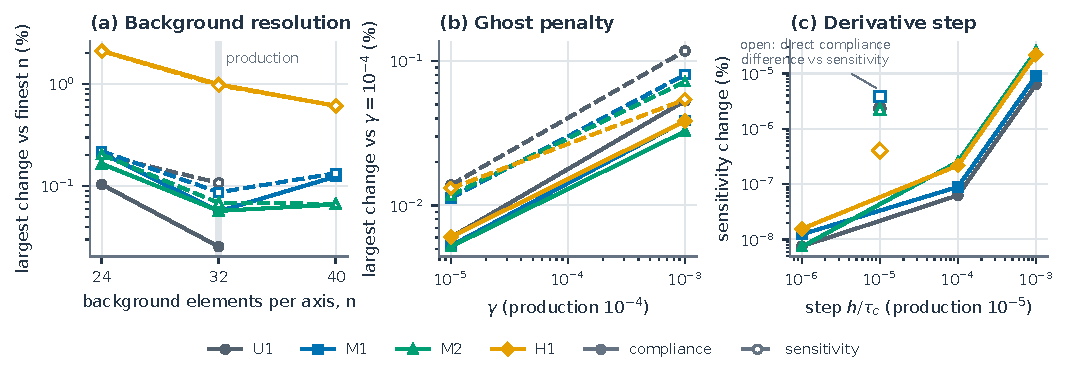
\includegraphics[width=\textwidth,height=0.8\textheight,keepaspectratio]{../figures/S06_reference_verification.pdf}
\caption{\textbf{CutFEM 参考解的验证。} 单个胞元在一个胞元表面上固支，并在另一个面上沿三个笛卡尔坐标方向分别受单位面力载荷作用。在 (a)、(b) 和 (d) 中，带实心标记的实线表示柔度，带空心标记的虚线表示厚度灵敏度，均取三个载荷下的最大相对变化。(a) 相对于所计算的最细背景分辨率的变化，U1 为 \(n=40\)，M1 和 M2 为 \(n=48\)；全文所用参考解取 \(n=32\)。(b) ghost 罚项系数偏离全文所用值 \(10^{-4}\) 时的变化。(c) 实心：矩导数的有限差分步长偏离全文所用值 \(h_c=10^{-5}\tau_c\) 时灵敏度的最大相对变化，在 \(10^{-3}\tau_c\) 处至多为 \(2.6\times10^{-5}\)\%，在 \(10^{-4}\tau_c\) 处再小一百倍；空心：在所用步长下，柔度中心差分与灵敏度之间的最大相对差异。(d) H1、H2 以及 NICE 误差最大（W1）和壁厚最薄（W3）的验证胞元加密至 \(n=64\)，数据见表 ST10；H2 没有 \(n=56\) 的解。}\label{fig:S01}
\end{figure}

\begin{figure}[!htbp]
\centering
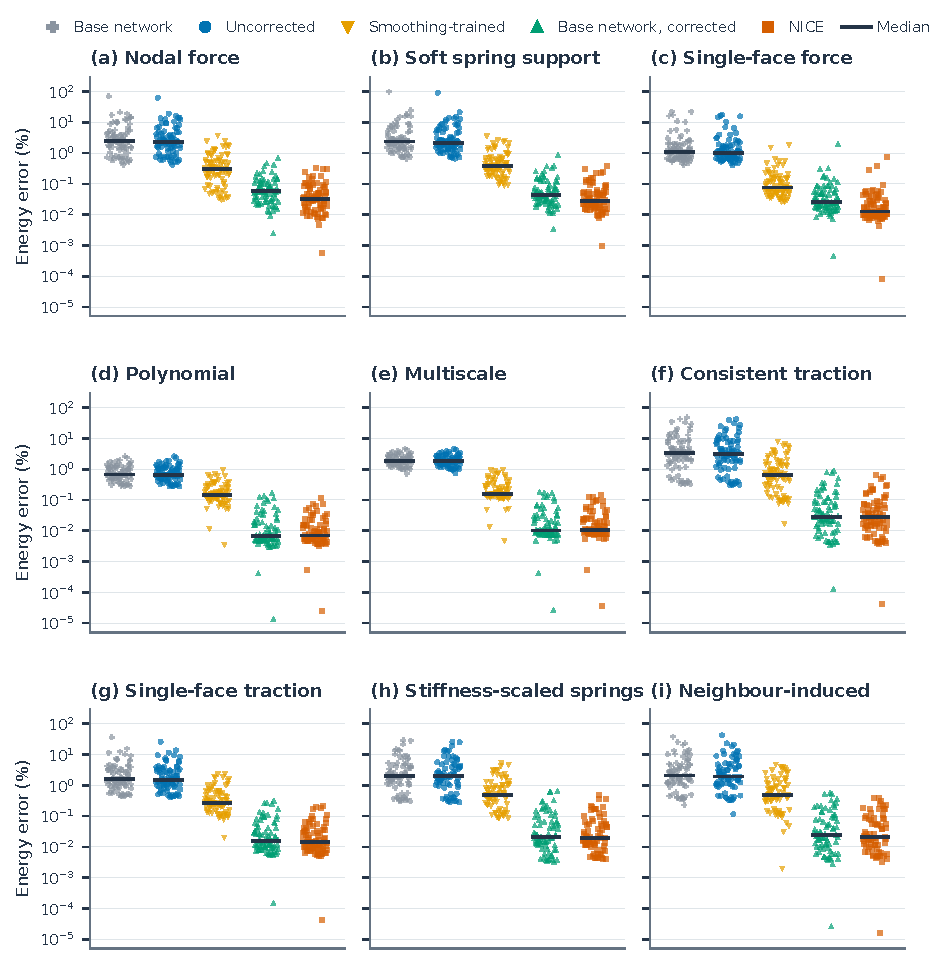
\includegraphics[width=\textwidth,height=0.8\textheight,keepaspectratio]{../figures/S01_distributions.pdf}
\caption{\textbf{几何层面能量误差的分布。} 每个点表示一个验证几何在恒等取向下的平均能量误差；水平短线为总体中位数。集中节点载荷、弹簧支撑、单面集中节点载荷、多项式位移、多尺度位移、面力载荷和单面面力载荷各类别包含 80 个几何。刚度缩放支撑类别和相邻胞元施加边界位移的类别各包含 75 个几何，与表 ST03 的总体相同。表 ST03 的五种变体（基础网络、未修正延续、平滑训练、基础网络加修正和 NICE）采用与正文图中相同的标记和颜色；基础网络加修正指在部署时对基础网络施加修正。以确定性的水平偏移区分重叠的观测点。所有子图共用对数误差轴。}\label{fig:S02}
\end{figure}

\begin{figure}[!htbp]
\centering
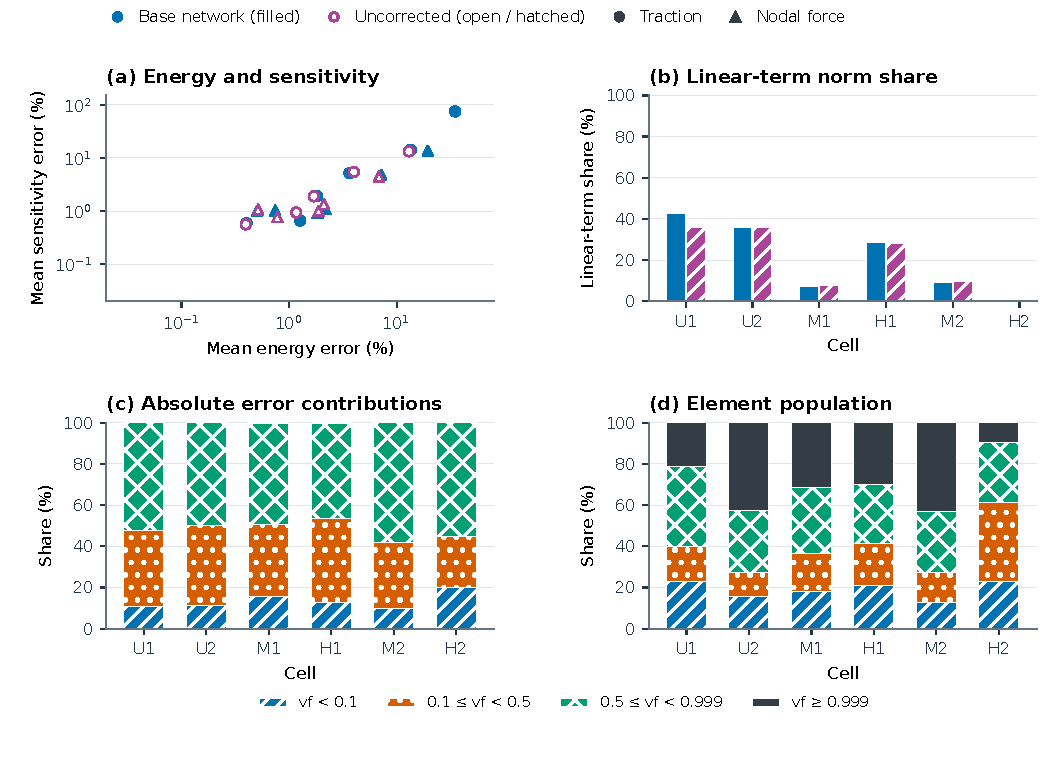
\includegraphics[width=\textwidth,height=0.8\textheight,keepaspectratio]{../figures/S03_sensitivity_diagnostics.pdf}
\caption{\textbf{灵敏度误差诊断。} (a) 面力载荷响应与集中节点载荷响应的平均能量误差与灵敏度误差配对，基础网络使用六个胞元，未修正延续使用五个胞元。(b) 面力载荷下线性项的范数占比 \(\|D_1\|_F/(\|D_1\|_F+\|D_2\|_F)\)，其中 \(D_1+D_2\) 为覆盖全部八个设计分量和所评估测试位移的灵敏度误差矩阵。(c,d) 基础网络在面力载荷下，四个互斥材料体积分数组中逐单元灵敏度误差绝对贡献的占比和单元数量占比。每个误差组先对其单元、设计分量和测试位移上的绝对贡献求和，再除以总和进行归一化。实心标记表示基础网络。在 (a,b) 中，空心标记和带阴影线的柱表示未修正延续；未修正延续给出了 U1、U2、M1、H1 和 M2 的结果（表 ST05a）。}\label{fig:S03}
\end{figure}

\begin{figure}[!htbp]
\centering
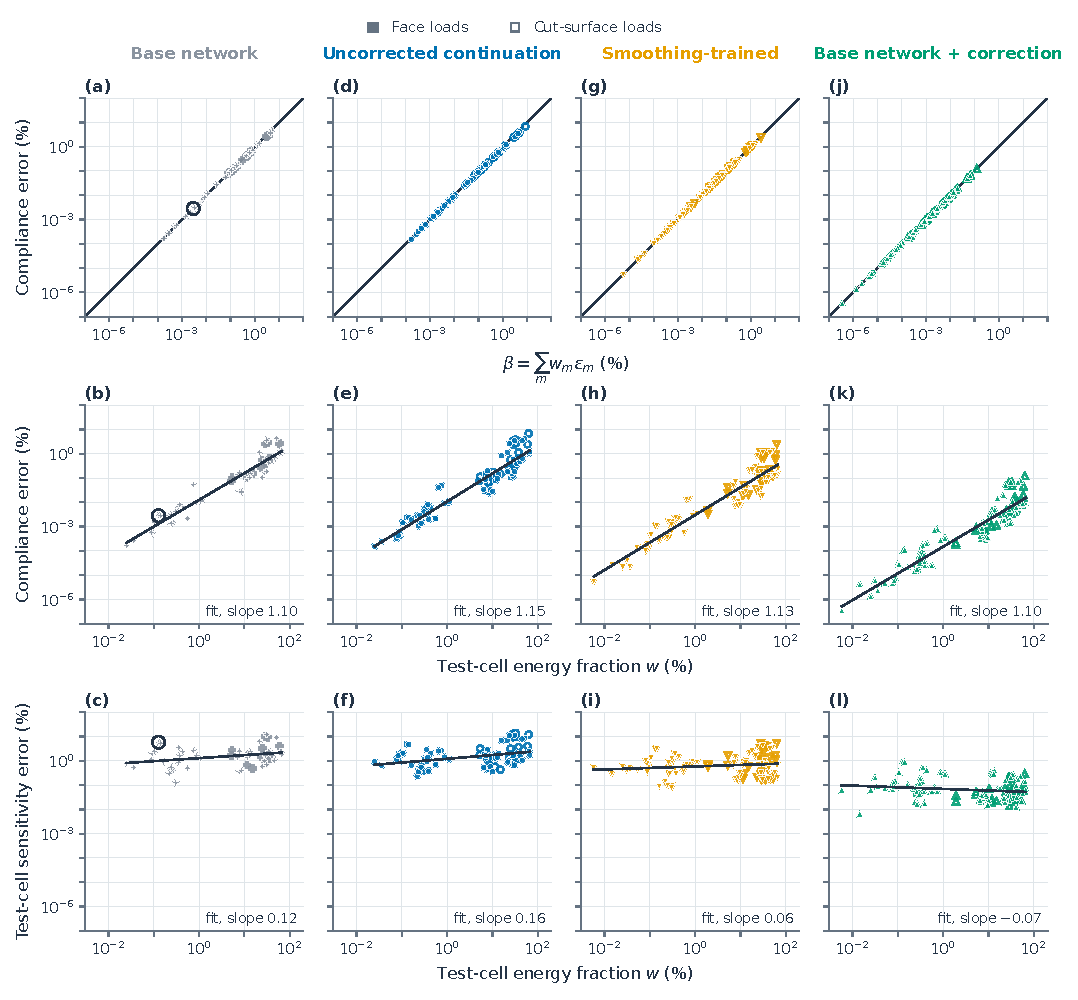
\includegraphics[width=\textwidth,height=0.8\textheight,keepaspectratio]{../figures/S07_energy_share_variants.pdf}
\caption{\textbf{其余四个变体遵循图 11 中的关系。} 与图 11 相对应，(a--c) 为基础网络，(d--f) 为未修正延续，(g--i) 为平滑训练变体，(j--l) 为基础网络加修正（部署时施加修正）。每个点对应各变体所评估构型中的一个载荷（分别为 54、87、96 和 114 个载荷；表 ST08 和表 ST09）；实心标记表示面载荷，空心标记表示切割面载荷。第一行：柔度误差与 \(\beta\) 的关系；直线表示相等。四个变体的柔度误差与 \(\beta\) 之比分别介于 0.80--0.98、0.79--0.99、0.92--0.99 和 0.96--1.006 之间；比值高于 1 的六个载荷，其超出量至多为柔度的 \(1.3\times10^{-9}\)。第二行和第三行：柔度误差和被测胞元灵敏度误差随被测胞元精确应变能占比 \(w\) 的变化；直线为对数坐标下的最小二乘拟合，各子图中标出其斜率。所有子图共用误差坐标轴。(a--c) 中圈出的载荷为 U1/x 在相邻胞元表面 z 向面力载荷作用下的情形，其数值见表 ST08 的说明。}\label{fig:S04}
\end{figure}

\end{document}
